%
%************************************************************************************
% Authors: Martin Nordio
% Created: March 2011
%
%************************************************************************************

%\documentclass[a4paper,12pt, twoside, english]{book}
\documentclass[a4paper,12pt, oneside, english]{mythesis}


\usepackage{nopageno}
\usepackage{latexsym}
\usepackage{graphicx}
\usepackage{xcolor}

\usepackage{fancyhdr}
\usepackage{hyperref}
\usepackage{xspace}
\usepackage{todo}
\usepackage{supertabular}
\usepackage{url}
\usepackage{amsfonts}
\usepackage{amssymb}
\usepackage{amsmath,bm}
\usepackage{makeidx}
\usepackage{semantic}

\usepackage{tabularx}

\usepackage{courier}

% for adding languages such as Java, C in listing and don't use verbatim
\usepackage{listings}
\usepackage{amsthm}

\usepackage{color}
\usepackage{enumitem}
\usepackage{pdfpages}
\usepackage{framed}
\usepackage[export]{adjustbox}

\setlength{\fboxsep}{0pt}

\definecolor{verylightgrey}{rgb}{0.95, 0.95, 0.95}

\definecolor{gray}{rgb}{0.4,0.4,0.4}
\definecolor{darkblue}{rgb}{0.2,0.2,0.8}
\definecolor{cyan}{rgb}{0.0,0.6,0.6}

\lstset{basicstyle=\scriptsize\ttfamily,breaklines=true}
%\lstset{backgroundcolor=\color{verylightgrey}}
\lstset{frame=lrtb}
\lstset{showstringspaces=false}


\lstdefinelanguage{XML}
{
  morestring=[b]",
  morestring=[s]{>}{<},
  morecomment=[s]{<?}{?>},
  stringstyle=\color{black},
  identifierstyle=\color{darkblue},
  keywordstyle=\color{cyan},
  morekeywords={xmlns,version,type}% list your attributes here
}

\lstset{% setup listings
    language=XML,% set programming language
        framextopmargin=2pt,
        framexbottommargin=2pt
}


%\lstset{framextopmargin=50pt}

% Eiffel Identifiers or expressions
\newcommand{\eid}[1]{\textsl{{\color[HTML]{000000} #1}}}
% Eiffel Class names
\newcommand{\ecl}[1]{\textsl{{\color[HTML]{3333FF} #1}}}
% Eiffel Keywords
\newcommand{\ekey}[1]{\textbf{{\color[HTML]{333399} #1}}}



%\graphicspath{{image/}} 
%\pagestyle{fancyplain}

\pagestyle{headings}
  

% with this we ensure that the chapter and section 
% headings are in lowercase 
\renewcommand{\chaptermark}[1]{\markboth{#1}{}} 
\renewcommand{\sectionmark}[1]{\markright{\thesection\ #1}} 

\frenchspacing

% George's $$ environment
\makeatletter
% ~ gives a \; space in math mode
\def~{\ifmmode\;\else\penalty\@M\ \fi}
%  Italic in mathematical formulas
\def\@setmcodes#1#2#3{{\count0=#1 \count1=#3
 \loop \global\mathcode\count0=\count1 \ifnum \count0<#2
 \advance\count0 by1 \advance\count1 by1 \repeat}}
\DeclareSymbolFont{italic}{OT1}{\rmdefault}{m}{it}
\let\mathit\undefined
\DeclareSymbolFontAlphabet{\mathit}{italic} \edef\@tempa{\hexnumber@\symitalic}
\@setmcodes{`A}{`Z}{"7\@tempa41} \@setmcodes{`a}{`z}{"7\@tempa61} \makeatother

% end George

\newcommand{\keyword}[1]{\hbox{\texttt{#1}}}

% definitions: Hoare triples, Eiffel keywords, etc
% ADD your definitions here
% For example: 


% Eiffel instructions:
\newcommand{\rescueInst}{\texttt{rescue}\xspace}
\newcommand{\rescue}{\texttt{rescue}\xspace}
\newcommand{\RetryInst}{\texttt{Retry}\xspace}
\newcommand{\debugInst}{\texttt{debug}\xspace}
\newcommand{\checkInst}{\texttt{check}\xspace}
\newcommand{\loopInst}{\texttt{loop}\xspace}
\newcommand{\ifInst}{\texttt{if}\xspace}
\newcommand{\thenInst}{\texttt{then}\xspace}
\newcommand{\elseInst}{\texttt{else}\xspace}
\newcommand{\fromInst}{\texttt{from}\xspace}
\newcommand{\rename}{\texttt{rename}\xspace}
\newcommand{\redefine}{\texttt{redefine}\xspace}
% Eiffel variables
\newcommand{\Retry}{\textit{Retry}\xspace}
\newcommand{\Result}{\textit{Result}\xspace}

\newcommand{\retryInst}{\texttt{retry}\xspace}



%\pagenumbering{none}


%\pagestyle{headings}

%\setlength{\hoffset}{1.0cm} 
%\setlength{\textwidth}{16cm}
%\setlength{\oddsidemargin}{1.1cm}
%\setlength{\evensidemargin}{-1.1cm}
%\setlength{\textheight}{23cm}

%\setlength{\hoffset}{-1.0cm} 
%\setlength{\textwidth}{16cm}
%\setlength{\textheight}{23cm}






\title{Your Title }

\author{\bf Your Name   \\
   \\
    ETH Zurich, Switzerland \\
    \texttt{your e-mail}  \ \\
}

\date{March 2011}





\begin{document}


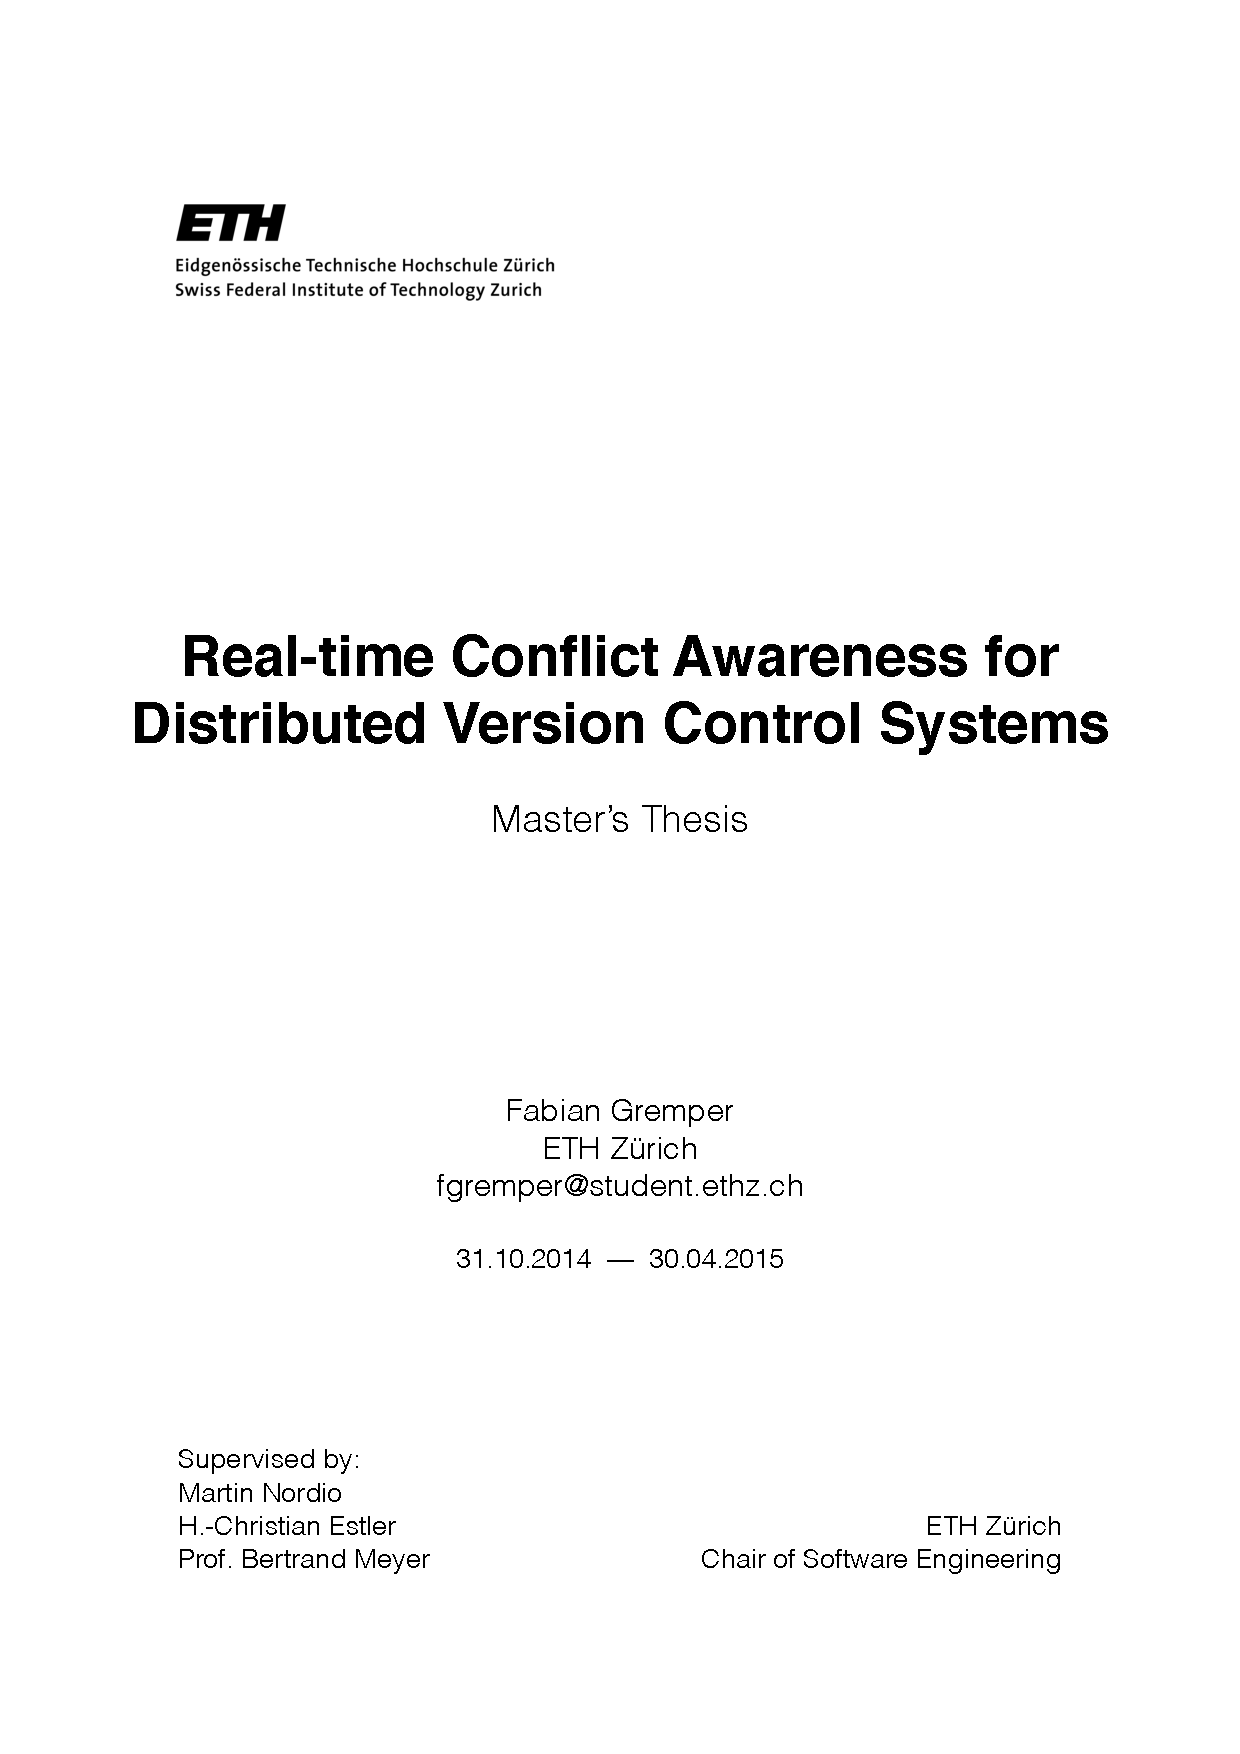
\includepdf[pages=-]{titlepage.pdf}

%\maketitle


%************************************************************************************
% Authors: Martin Nordio
% Date: March 2011
% Root file: report_root.tex
%************************************************************************************



\chapter*{Abstract}

\textbf{In this day and age, most computer programs are written by a team of more than one person. Because software engineering is becoming increasingly distributed, we require smart mechanisms and systems to reduce overhead and stress introduced by a lack of awareness and the need to resolve conflicts.} \\

\textbf{This thesis introduces a new tool for users of a distributed version control system: CloudStudio is an awareness system for Git, providing information about "who is working on what" and possible conflicts through a publicly available API. This allows developers to integrate this information in new ways, e.g. directly as a plugin for common IDEs. CloudStudio can work with all Git repositories and does not require a specific project setup.} \\

\textbf{CloudStudio divides awareness information into three distinct views: branch view, file view and content view, with each view serving a different purpose and separating the information in a way that?s easily understandable for users. Many options and filters can be used in all views to enhance the view for specific needs and make sure you find what you are looking for.}

% 1. What is the problem? 
% 2. Why is this problem interesting/relevant?
% 3. What is our solution approach?
% 4. What did we achieve?




%************************************************************************************
% Authors: Martin Nordio
% Date: March 2011
% Root file: report_root.tex
%************************************************************************************



\chapter*{Acknowledgements}

I would like to thank Prof. Dr. Bertrand Meyer for giving me the opportunity to realize my master thesis at the Chair of Software Engineering. \\

I would like to express my gratitude to my supervisors Dr. Martin Nordio and H.-Christian Estler for their great support throughout my work on this master thesis.


% 1. What is the problem? 
% 2. Why is this problem interesting/relevant?
% 3. What is our solution approach?
% 4. What did we achieve?



%\newpage

\tableofcontents




\pagenumbering{arabic}




%************************************************************************************
% Authors: Martin Nordio
% Date: March 2011
% Root file: report_root.tex
%************************************************************************************


%----------------------------------------------------------------------------
\chapter{Introduction}\label{introduction}
%----------------------------------------------------------------------------

\section{Distributed Software Development}

Today's software projects are increasingly distributed across multiple locations over all of the world \cite{ref1, ref2}.  This distribution poses new challenges to software development, especially those related to collaboration, as globally distributed development is necessarily collaborative  \cite{ref3}. \\



Many researchers have evaluated the effect of distributed software development  \cite{ref5, ref6, ref8} and suggested that providing awareness information about who is making what changes may greatly reduce overhead generated by conflict resolution and overall improve the effectiveness of collaboration  \cite{ref3, ref4}. \\



Studying the difficulties in communication and collaboration are of utmost importance  \cite{ref10, ref2}. The aspects of software development distribution have been researched from many angles  \cite{ref14, ref15, ref10}. Nordio et al. have researched the impact of contracts in distributed software development to mitigate the risk of misunderstanding software specifications  \cite{ref9}, as well as the impact of distribution and time zones on  communication and performance in distributed projects [16]. \\



Over the course of several years of teaching "Distributed and Outsourced Software Engineering" (DOSE), Nordio et al. have studied key characteristics in improving collaborative development and have found that the emphasis on API design and development of communication skills are among the leading factors, since at least 30\% of the time spent by students in the project has been found to correspond to communication \cite{ref19, ref20}.

\section{Version Control Systems}


Version Control Systems (VCS) are widely used in almost all projects with multiple team members. \\

"In traditional version control systems, there is a central repository that maintains all history. Clients must interact with this repository to examine file history, look at other branches, or commit changes. Typically, clients have a local copy of the versions of files they are working on, but no local storage of previous versions or alternate branches. \\

Distributed Version Control Systems (DVCS) such as Git and Mercurial have becoming increasingly more popular during the last few years. With DVCS, every user has an entire copy of the repository locally; switching to an alternate branch, examining file history, and even committing changes are all local operations. Individual repositories can then exchange information via push and pull operations. A push transfers some local information to a remote repository, and a pull copies remote information to the local repository." \cite{ref17}




\section{Awareness and Conflict Detection}





Conventional version control provides a means to collaborate on writing programs, even different subtasks, and merge the changes later. Merging changes can however produce conflicts. To avoid big conflicts, we want to provide the programmer with an awareness system to inform them at the time of writing if another programmer is currently editing parts of the code that may be conflicting with their current work. \\

Researches have found that interruptions due to insufficient awareness occur frequently for teams of non-trivial size. A large and diverse set of information items has been found to be very important if they are related to the project a distributed software engineer is currently working on \cite{ref21}, while developers often have different preferences regarding the frequency and detail that awareness information should have \cite{ref3}. 




\section{Motivation}




With the increasing importance on distributed software development, it has become necessary to construct techniques and tools that can assist programmers to make them more productive in such an environment \cite{ref13}. CloudStudio is a collaborative development framework proposed by Nordio et al. \cite{ref12, ref28} where the software configuration management, conflict detection, and awareness systems are unitarily conceived and tightly integrated. \\

This thesis is a proposal at a new software solution, built from ground up, to provide programmers with extensive and relevant awareness information and a mechanism to detect possible conflicts early. I was asked to keep the name CloudStudio for this project. In this section, I will describe some of the differences and aspects that I am trying to improve with my thesis. For this purpose I will refer to my new version as CloudStudio 2.0, and to the previously existing implementation as CloudStudio 1.0. \\

CloudStudio 1.0 is a web-based IDE that allows users to work, collaborate and run code directly in the browser. Behind the curtains, CloudStudio 1.0 sets up a new Git repository for every project that is used for its intrinsic version control. \\

The web interface and the functionality of the CloudStudio 1.0 server and deeply intertwined. The system is designed for users to solely work through the web interface and does not provide an API to directly request awareness information from the server, for example to allow inclusion of CloudStudio's awareness features in widely used IDEs, such as EiffelStudio \cite{ref26} or Eclipse. CloudStudio 2.0 offers an extensive API for this purpose and its web interface communicates directly through this API. \\

More importantly, CloudStudio 1.0 is dependent on a specific Git repository setup that it creates initially when a new CloudStudio project is created. It is not possible to use any of its functionality with pre-existing Git projects that were not specifically set up in CloudStudio in the first place. While it is possible to retrieve a CloudStudio 1.0 project's Git repository from the backend, perform some work directly on the Git repository and push it back to the server, there are many limitations: e.g. you would be required to follow its internal branch naming conventions and all awareness queries would still have to be done through the web interface. \\

A big focus of CloudStudio 2.0 is also robustness to possible errors, deviation in repository structures and invalid requests. \\

With this in mind, CloudStudio 2.0 uses a different approach from its predecessor and has been built from ground up during the course of this master thesis. The next section, as well as section \ref{designfeatures} will cover the details and features of the new implementation. From this point on, CloudStudio will refer to this implementation.







\section{Goals}




This project focuses on creating a useful mechanism for users of a distributed version control system to detect possible conflicts early on and provide them with awareness information about who is changing what. \\

There are several components that are being implemented in order to achieve this:


\begin{itemize}

\item A CloudStudio client that needs to run on each developer's machine will gather information about the local Git repository and local working tree and sends relevant information to the CloudStudio server periodically.
\item The CloudStudio server will then use the data from all the users running the plugin, as well as the data from a central remote repository (origin) to detect possible merge conflicts that may occur at some point when two or more parties attempt to push their changes. CloudStudio server will also provide extensive awareness information about who is changing what and the current state in which the users are in relation to the central remote repository.
\item The CloudStudio server will then provide a well defined API that allows other programs or tools to retrieve this awareness information.
\item A web interface will be implemented to access and demonstrate CloudStudio's awareness capabilities.

\end{itemize}

There are many subgoals to this project:

\begin{itemize}

\item The API should be well defined and well documented. In the future, instead of only the web interface, it is conceivable that CloudStudio's awareness information could be also made available directly in the users' IDE through a plugin.
\item Awareness information generated by CloudStudio is correct and useful.
\item CloudStudio acts as a separate layer on top of Git. Its functionality can be added to existing projects without the need to make any changes to the structure of the Git repository.
\item The implementation of all parts should be robust and stable; errors should be dealt with appropriately.
\item CloudStudio should be user-friendly and easy to use.

\end{itemize}

Under section 2.1.1 the features of CloudStudio are listed in detail.







\section{Related Work}




Extensive research in the area of awareness has spawned other tools seeking to raise developers' awareness about the changes introduced by others. The granularity of awareness information varies from tool to tool. \\

Crystal is a publicly-available tool that uses speculative analysis to make concrete advice unobtrusively available to developers, helping them identify, manage, and prevent conflicts. \cite{ref25} \\

Syde is a a tool to reestablish team awareness by sharing change and conflict information across developers' workspaces \cite{ref23}. It uses the abstract syntax tree (AST) to detect conflicts and apply change awareness on the syntax level and was used to investigate conflict detection in a user study \cite{ref24}. \\

Palantir is an Eclipse plug-in to address direct and indirect conflicts, which arise due to ongoing changes in one artifact affecting concurrent changes in another artifact \cite{ref22}. \\

FASTDash is an interactive visualisation tool that seeks to improve team activity awareness using a spatial representation of the shared code base that highlights team members' current activities. It provides file-level awareness of the activities in Visual Studio projects \cite{ref26}. \\

Jazz is an Eclipse plugins that shows simple change awareness by highlighting changed lines, designed to support small, informal teams; anyone can create a team and add or remove members \cite{ref27}. \\

And of course, the already mentioned original CloudStudio, a web-based framework that sharing the changes of developers working on the same project; its real-time awareness system allows for dynamic views on the project by selectively including or excluding other developers' changes \cite{ref12}.





%************************************************************************************
% Authors: Martin Nordio
% Date: March 2011
% Root file: report_root.tex
%************************************************************************************


%----------------------------------------------------------------------------
\chapter{Design}\label{design}
%----------------------------------------------------------------------------


\section{Introduction}


The following subsections discuss the features that I want CloudStudio to provide and how these features can greatly improve the collaboration experience for users, as well as the approach behind the implementation of CloudStudio.


\subsection{Features}\label{designfeatures}

CloudStudio provides numerous awareness and conflict detection features that users can benefit from. The following is a list of provided awareness information:


\begin{itemize}


\item an overview of all users and their relative commit position in relation to the origin. This can show you if users have recently synchronized with the origin, are behind or have made local commits in the meantime.
\item the branch that is currently checked out by each user in a project, refered to as the "active branch". This helps users to coordinate their work, especially in big teams with many feature branches for subfeatures.
\item the last time since information has been updated for each user, so you never run into the risk of relying on outdated information.
\item the last time since CloudStudio has updated its data from the central remote repository (e.g. GitHub)
\item from your perspective, what files have been modified by other users, and if so, whether a push by both parties would result in a merge conflict
\item from the perspective of the origin, what files have been modified by which users. If multiple users are working on the same file, it may be appropriate to coordinate further implementations.
\item the possibility to stage the same conflicts, but from the perspective from your user in one branch and all other users in another branch. This will highlight changes or conflicts that would occur in the future when these branches are going to be merged together.
\item possibility to view either locally committed changes or changes made in the local working tree that have not yet been locally committed. For the latest status information you may want to view uncommitted changes; this may bring up changes that are possibly not meant to be checked in at any point and are just experimental. The latest locally committed changes, however, are going to be pushed to the origin at some point.
\item a detailed side-by-side comparison of two versions of a file for two different users, one of which may be the origin.
\item a detailed side-by-side merge conflict view for two versions of a file for two different users. In this view, a common ancestor is used as a reference for a three-way merge and will show the same conflicts that would occur when Git tries to merge the files.
\item numerous filters that can enhance or narrow down your view to information that is interesting to you: filtering by users allows you to only look at a subset of users, filtering by conflict severity will only show conflicts above a certain threshold.
\item grouping awareness information by folders lets you monitor subprojects as a whole.

\end{itemize}



\subsection{Approach}\label{designapproach}


CloudStudio can be thought of as an extra layer on top of an existing Git repository setup. There are no requirements for a specific setup in the Git repository and it can work with existing, as well as new projects and provide extensive awareness information and detect possible conflicts. CloudStudio is divided into two primary parts: a server and a client. \\

The client is a standalone tool that has to be run in the background by all users in a project that want to benefit of the added awareness information provided by CloudStudio. It will send data to the server periodically and can work with multiple local repositories that are working with the same CloudStudio server. The client provides a graphical user interface that show its current state and its actions to the user. \\

The server is hosted at a publicly available host and port and can deal with many users, many repositories and provides a central, single-login based structure to send and retrieve awareness information to and from. Through a public and well-documented API, this awareness information can be easily integrated with existing IDEs, such as EiffelStudio \cite{eiffelstudio} or Eclipse, or be used in any desired form. For this thesis, a web interface is being implemented and provides access to all the awareness features directly in the browser. \\

Graphic \ref{fig:typicalsetup} shows a typical setup for a single repository: many clients are working on a project using local Git repositories that are synchronized with each over through a central remote repository. Additionally, all users run a CloudStudio client, that will provide the CloudStudio server with the information necessary for it to prepare its awareness information. This way, the two parts function independently from each other and the underlying repository structure is not affected by using CloudStudio. It also means that the central repository can be hosted anywhere (e.g. GitHub) and can still be used with CloudStudio. \\

\begin{figure}[h!]
  \centering
      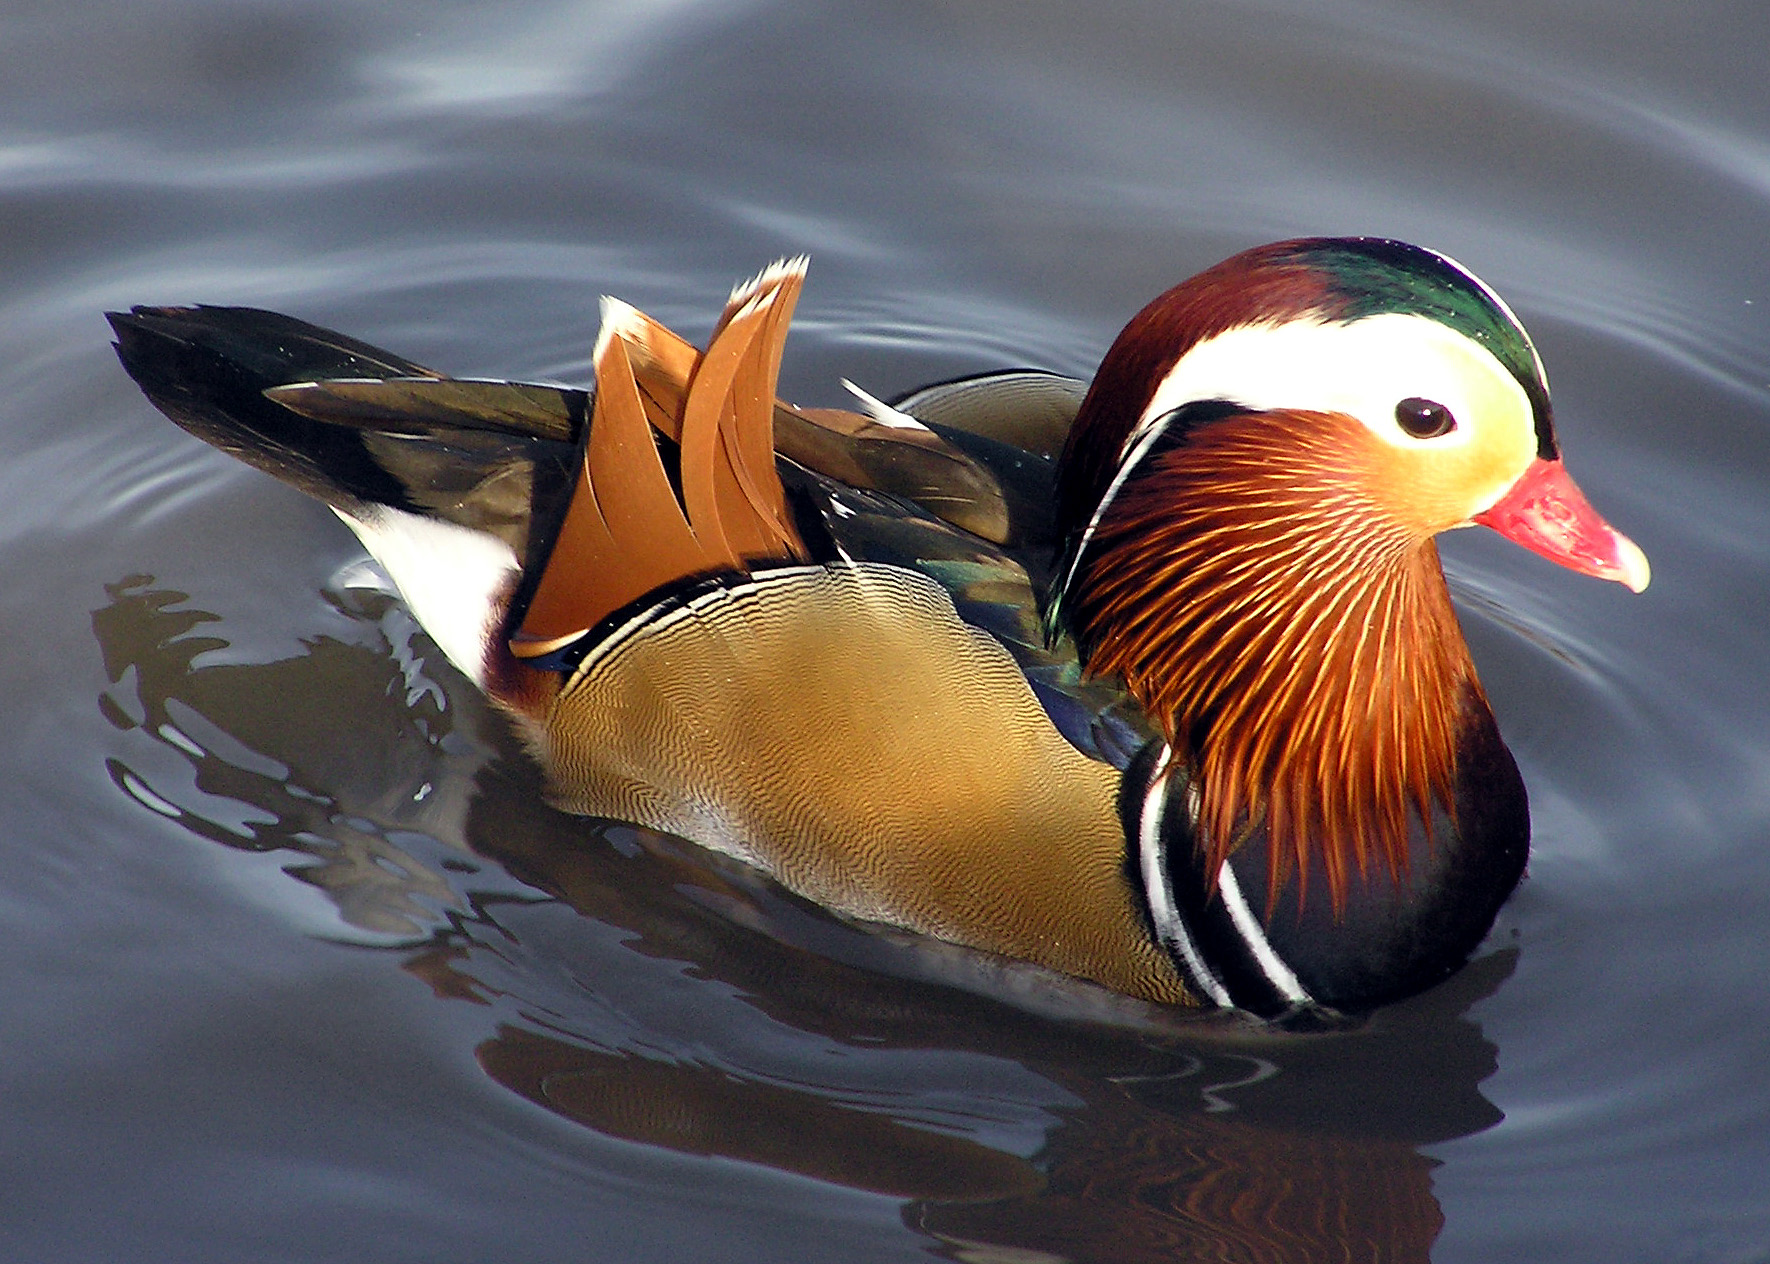
\includegraphics[width=1\textwidth]{generalsetup}
  \caption{Typical CloudStudio setup for a single repository}
  \label{fig:generalsetup}
\end{figure}

Both parts, client and server, are highly customizable through an XML-based configuration file. The configuration is explained in detail in section \ref{configmanagement}.






\section{Separation of Awareness Views}

Awareness information is separated into three different views: branch view, file view and content view. Each view provides distinct information and servers its own purpose; however, some information can be accessed in an overlapping manner, if desired. The views are also built in a way that there is a natural flow for users to navigate from more broad to more detailed information in a repository. \\

The following sections discuss the functionality and purpose of each view in detail.







\section{Branch Level Awareness}




The branch level awareness view is the first view in the navigation sequence for a given repository. \\

One of the most important awareness features of this view is the display the local commit state of all users in relation to the origin. In Git, every commit has a unique identifier and all commits are arranged in a graph with each commit having a pointer to a parent commit, making up a directed graph of all commits. While a local repository may not know about all possible commits of all users, we can reconstruct this information using the data sent by the CloudStudio client. \\

Using this information, the CloudStudio server uses one of the following values to describe each users relationship with the origin: $equal$, $ahead$, $behind$, $fork$, $local$ $branch$, $remote$ $branch$. In case of $ahead$, $behind$ or $fork$ we are also given a distance. I will demonstrate the meaning behind these values using an example. \\

Let Figure \ref{fig:usercommitstructure} represent the commit history graph for a repository and four users; every commit is shown as a green box with a commit ID. For every user and branch, a reference points to a specific commit, indicating the commit that we are working on when we are working on a specific branch. The origin also has pointers to a single commit for every branch. The combined commit graph created from all of these individual local commit graphs is seen in Figure \ref{fig:combinedcommitstructure}.


\begin{figure}[h!]
  \centering
      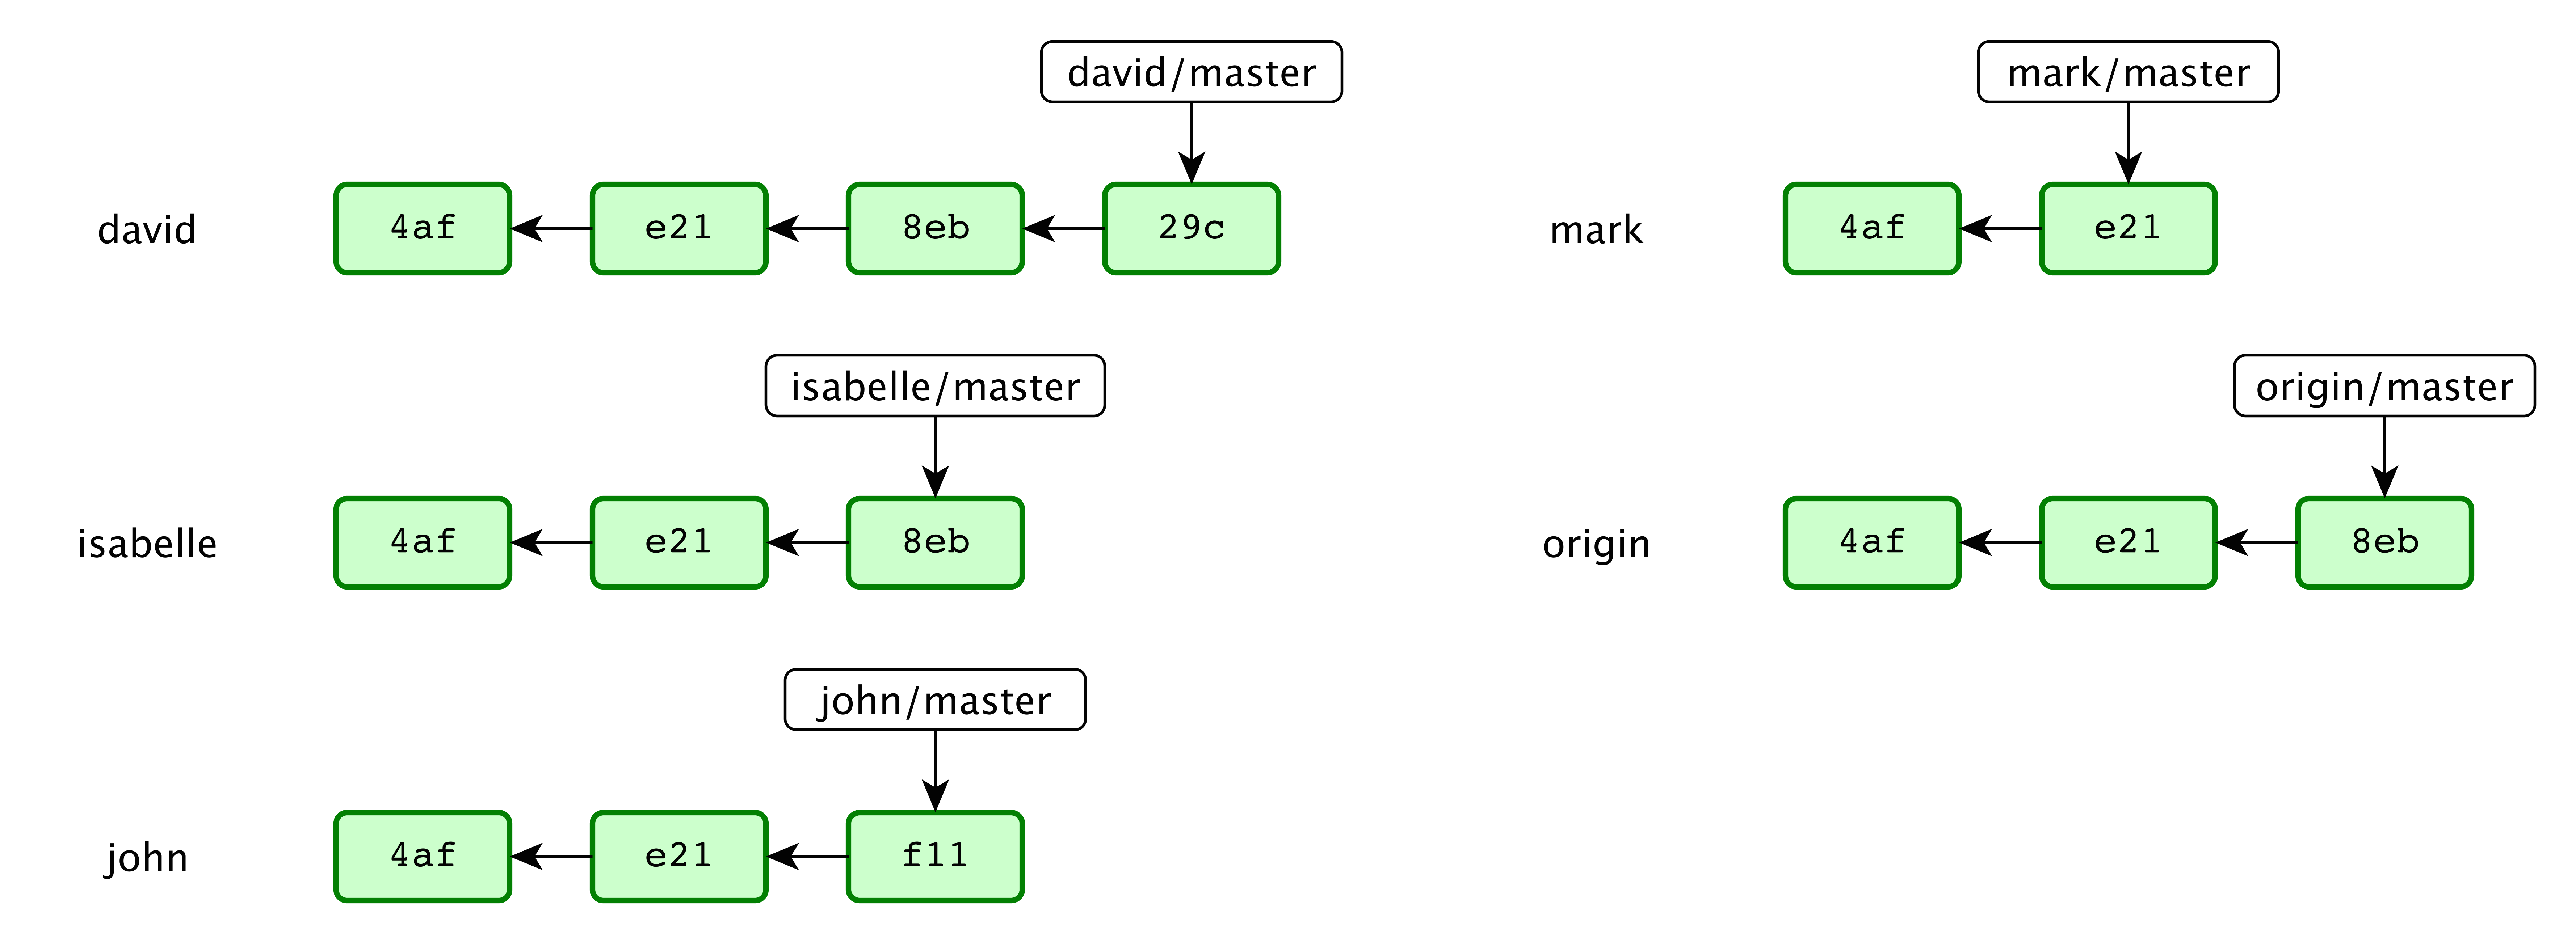
\includegraphics[width=1\textwidth]{commitgraph1}
  \caption{Commit history graph for users in a system}
  \label{fig:commitgraph1}
\end{figure}


\begin{figure}[h!]
  \centering
      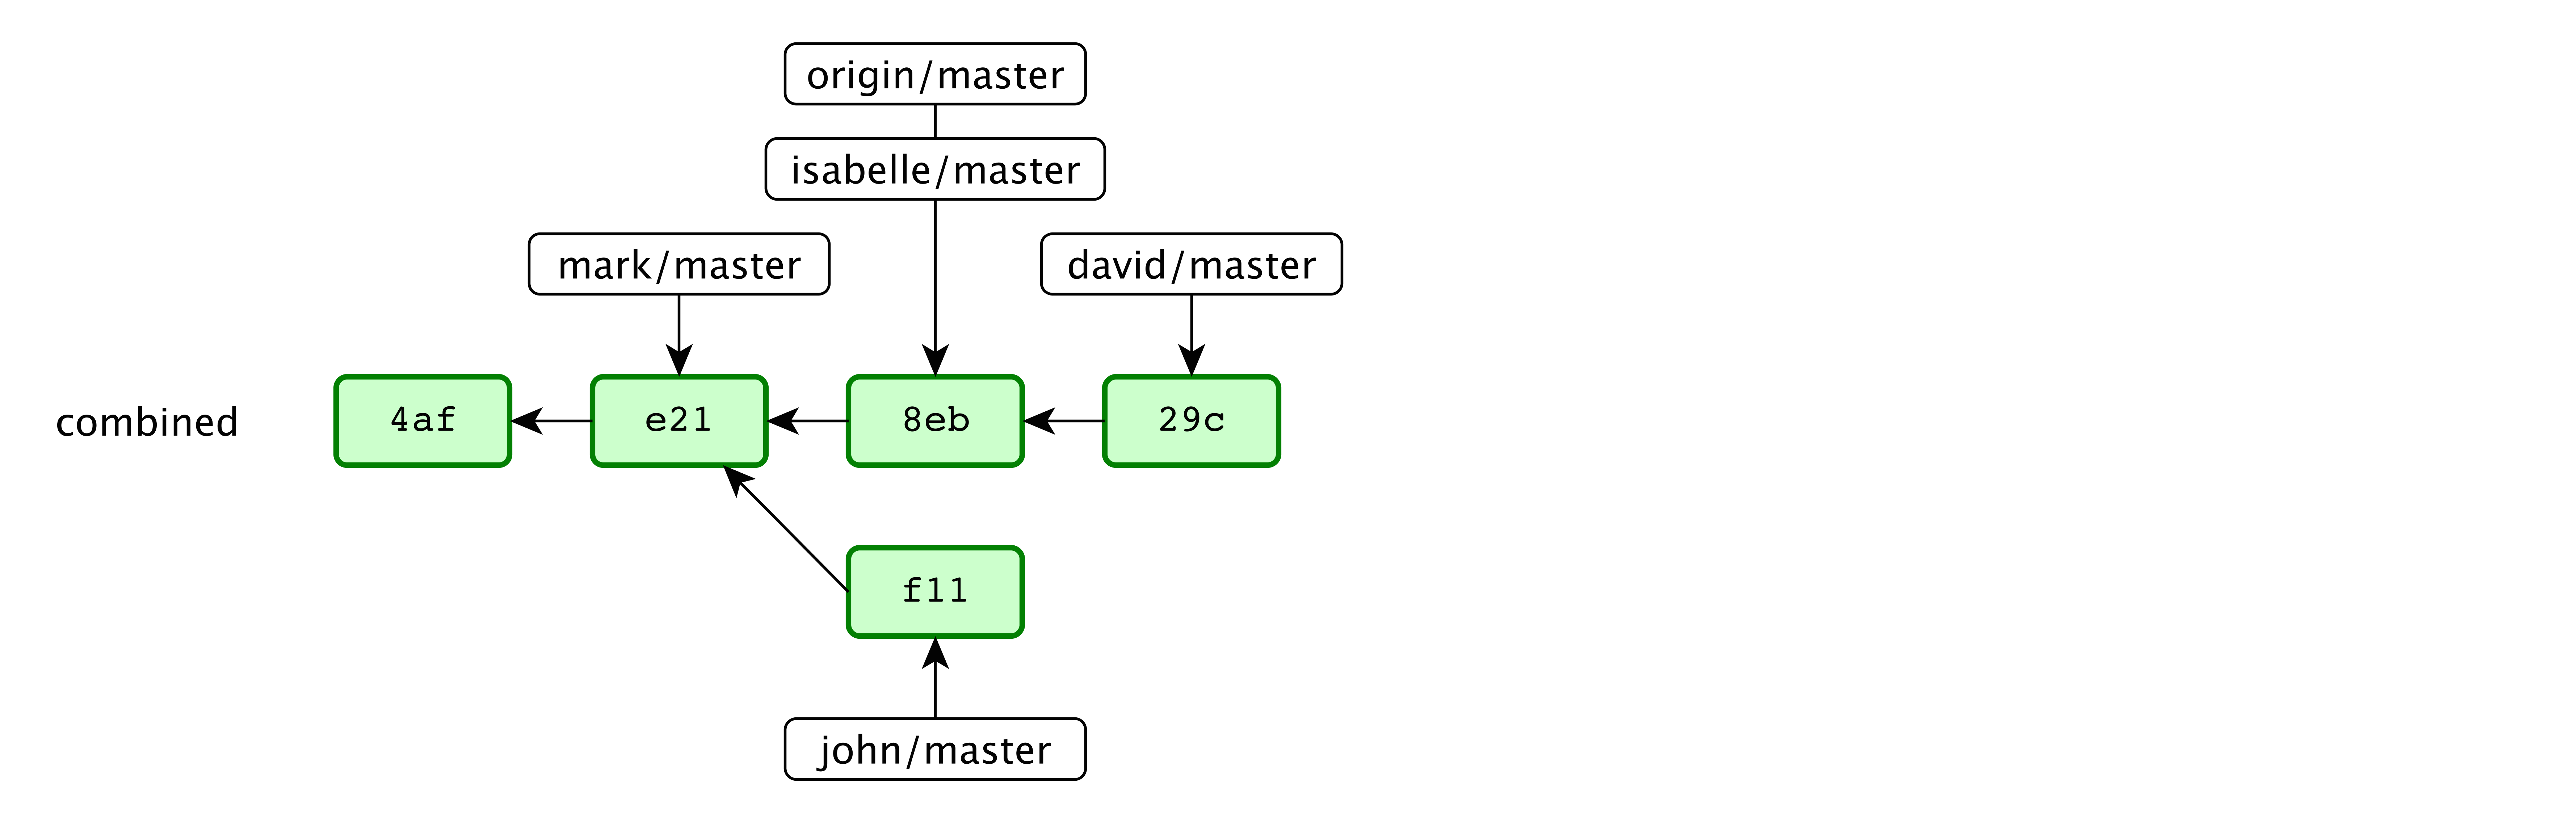
\includegraphics[width=1\textwidth]{commitgraph2}
  \caption{Combined commit history graph}
  \label{fig:commitgraph2}
\end{figure}

From this graph we can deduct the following relationships:

\begin{itemize}


\item Isabelle is $equal$ to the origin. Her local repository is up to date and she has not made any further local commits.
\item David has made a new local commit after his last repository pull and has one local commit that he hasn't pushed to the origin yet. He is $ahead$ of the origin, with a distance of 1 because he needs to traverse one edge in the graph to reach the commit that the origin is pointing to. David could at this point push his changes to the origin and the origin would simply fast-forward merge, meaning it will add the new commit and point its $master$ branch reference to \texttt{29c}.
\item Mark is $behind$ the origin; he has pulled from the origin when \texttt{e21} was the active commit and has not pulled or made a local commit since.
\item John is in a $fork$, with a distance of 2, as he has also last pulled from the origin at \texttt{e21} but has made a local commit (\texttt{f11}). In the meantime someone (either Isabelle or David, given the commit graph) has made a commit (8eb) and pushed it to the server. If John was to push to the server, a merge between \texttt{8eb} and \texttt{f11} would be made and stored in a new commit.

\end{itemize}


The same reference pointers that the example shows for the master branch are also given for all other branches in the system and the calculations behave analogous. If a user has a branch pointer for a branch that isn'tt on the origin, the relationship is given as $local branch$; for a branch that only exists on the origin but not in a users local repository, the relationship is $remote branch$. \\

This awareness feature only deals with locally committed changes and is a useful measure of how up to date local repositories are in relation to the origin. If a user is a $behind$, they should perform a pull. If they are $ahead$, they should push their changes. If they are in a $fork$, it means they started working on a feature while in the meantime someone else pushed their local changes; this case will necessarily result in a merge. $Forks$ will occur often, usually right before pushing, as the only way to avoid them is if only one user is making a change at the time. A low distance can indicate that fewer changes have been made, while a high distance can indicate a big amount of changes. \\

For each branch in this view, a list of active users is given. If a user has currently checked out a specific branch into their local working tree, it is their "active repository" and indicates they are working on it. This is very useful to get an overview of what all users are working on, especially if branches have meaningful names (e.g. ticket identifier for feature tickets) and there are many users in a project. \\

A timestamp shows the last time that the user has updated their state via the CloudStudio client and indicates how recent and accurate the provided information is for each user. This way, users do not falsely rely on outdated information.






\section{File Level Awareness}

As the second step in a usual navigation path through the awareness system, the file level view shows awareness information and possible conflicts for all files in a repository. This is achieved by doing a pair-wise comparison of your version of a file with all the version of all users in this branch. Alternatively you can also choose to view differences from the origin's point of view.

In its basic form, the file level awareness view compares file checksums to find out whether a file has been modified. If the two file versions that are being compared are not identical, this is presented as a file conflict. It should be noted that non-existing files are treated as empty files for the purpose of this comparison.


\subsection{View as Origin}

If you are viewing from the origin's point of view, a file conflict indicates that the latest version in the remote repository and a user's local file differ; speaking in terms of awareness: all users that are shown up as conflicting have changed their file locally and are probably working on it. If you choose to show uncommitted changes, it will compare the most up to date version of a file from each user's working tree; otherwise it will use the latest committed version. \\

This viewpoint provides useful awareness information to see what users are working on what file. If multiple users show up as a file conflict for the same file, they should coordinate their changes early in order to avoid merge conflicts later on.

\subsection{View as Yourself}

By not using the "view as origin" option, your local files are compared directly to all other users'. However, a file conflict is less meaningful here: if you have changed a file, all other users will show up as a file conflict because the file checksums differ. More interesting in this case is to enable the "show conflicts" option.

\subsection{Show Conflicts}

With the "show conflicts" option enabled, the comparison does not directly compare the two file versions, but instead does a three-way comparison by taking the nearest common ancestor of both files from the commit history as the baseline. This emulates the same behaviour that Git would do when performing a merge: Git will select a merge base and try to merge files automatically if different portions of the file have been changed. In this three-way comparison, a merge conflict would by definition occur only, if in some part either all three files differ, or if only the base file differs. \\

For all the files and users that would show up as file conflicts (without this option enabled), this three-way comparison will additionally look for merge conflicts and mark files that would not pass an automatic merge as content conflict. This is very useful, because when two users are working on a file simultaneously but they are working on different parts, no content conflicts are shown. As soon as they are changing the same portions of a file and Git would have trouble merging the files at a later point, a content conflict is displayed. This helps catching merge conflicts very early on and users can arrange their work and take countermeasures early before the merge overhead becomes bigger.

\subsection{Compare to Other Branches}

The same functionality can not only be used to show branch internal awareness and conflict information---by specifying a different comparison branch, your (or the origin's) files from your selected branch are compared with all other users' in the specified branch. \\

Let's say you are working on the master branch and someone else is called on a feature branch "iss53" that will have to be merged into the master branch at a later point in time.

By selecting branch comparison with "iss53" from the viewpoint of the master branch, you can see file and content conflicts that will occur when merging your local master branch state with each other user's iss53 branch state. Likewise, by comparing with the master branch from iss53's point of view, the comparison will be made between your files from the master branch with all other users? files in the iss53 branch. \\

In the same manner, the comparison functions with the "view as origin" option enabled: instead of your files from the selected branch, the files from the origin will be compared.

\subsection{Filters}

You can choose to filter your view by only selecting a subset of the users in a project. If the number of users is really big, this helps narrow down your search and display only information relevant to you.

It is also possible to filter files by the severity of conflicts. Selecting "content conflicts" only shows files and users with a conflict type of "content conflicts", "file conflicts" shows both file and content conflicts, an no filter also shows users and files where the files are equal.

\subsection{Grouping}

Folders have a grouping mechanism that add up the containing conflicts. If a user contains at least a content conflict, it will be marked as a folder containing content conflicts and the users responsible for it will be listed. Likewise file conflicts propagate their conflict type up to the containing folders.

\subsection{Uncommitted vs. Committed Files}

As already mentioned above, you can always select to work either with locally committed files or uncommitted files directly from the active working tree from all users. Working with uncommitted files has the advantage of always have the latest version of all files, while you are running into the risk that these changes may not be final or only experimental and will never make it into an actual commit. Viewing committed files is more safe in this regard, but may not show very recent changes.







\section{Content Level Awareness}




The content level awareness view allows you to compare two versions of a file side-by-side. \\

In non-conflict mode, files are compared side-by-side directly and insertions, deletions and modifications are highlighted. \\

In the conflict mode, the closest common ancestor in the commit history is taken as a base file for a three-way comparison. The comparison is done using the diff3 algorithm that is also used by Git to internally merge files automatically. Sections of the file are matched into blocks; if a block has been changed in all three files or only in the base file, a conflict occurs, because a three-way merge could not automatically decide how to merge these files together. These conflicts are highlighted in red, while normal modifications that would be merged automatically by Git are shown in light blue. \\

The content awareness view allows you to toggle the options to show uncommitted files, show conflicts and view as origin directly in place.










%************************************************************************************
% Authors: Martin Nordio
% Date: March 2011
% Root file: report_root.tex
%************************************************************************************


%----------------------------------------------------------------------------
\chapter{Implementation}\label{implementation}
%----------------------------------------------------------------------------



\section{Introduction}

CloudStudio consists of three distinct implementation parts at this point: the server, the client and the web interface. The server and client are both written in Java, while the web interface runs in JavaScript. \\

The client periodically sends data to the server to keep the awareness information of CloudStudio up to date. The server provides a public API to request awareness information directly, as well as a user-friendly web interface that uses and showcases the full capabilities of the API. \\

The server provides a central login system for its users and allows them to work with Git repositories hosted independently from CloudStudio. \\

A MySQL database stores all of the data; its details are explained in section \ref{database}.





\section{Architecture}

\subsection{Architectural Overview}

While in \ref{designapproach} the entire system was presented from a global point of view, this section deals with the internal architecture of CloudStudio system. Figure \ref{fig:entities} shows an architectural overview of all entities in CloudStudio. \\

\begin{figure}[h!]
  \centering
      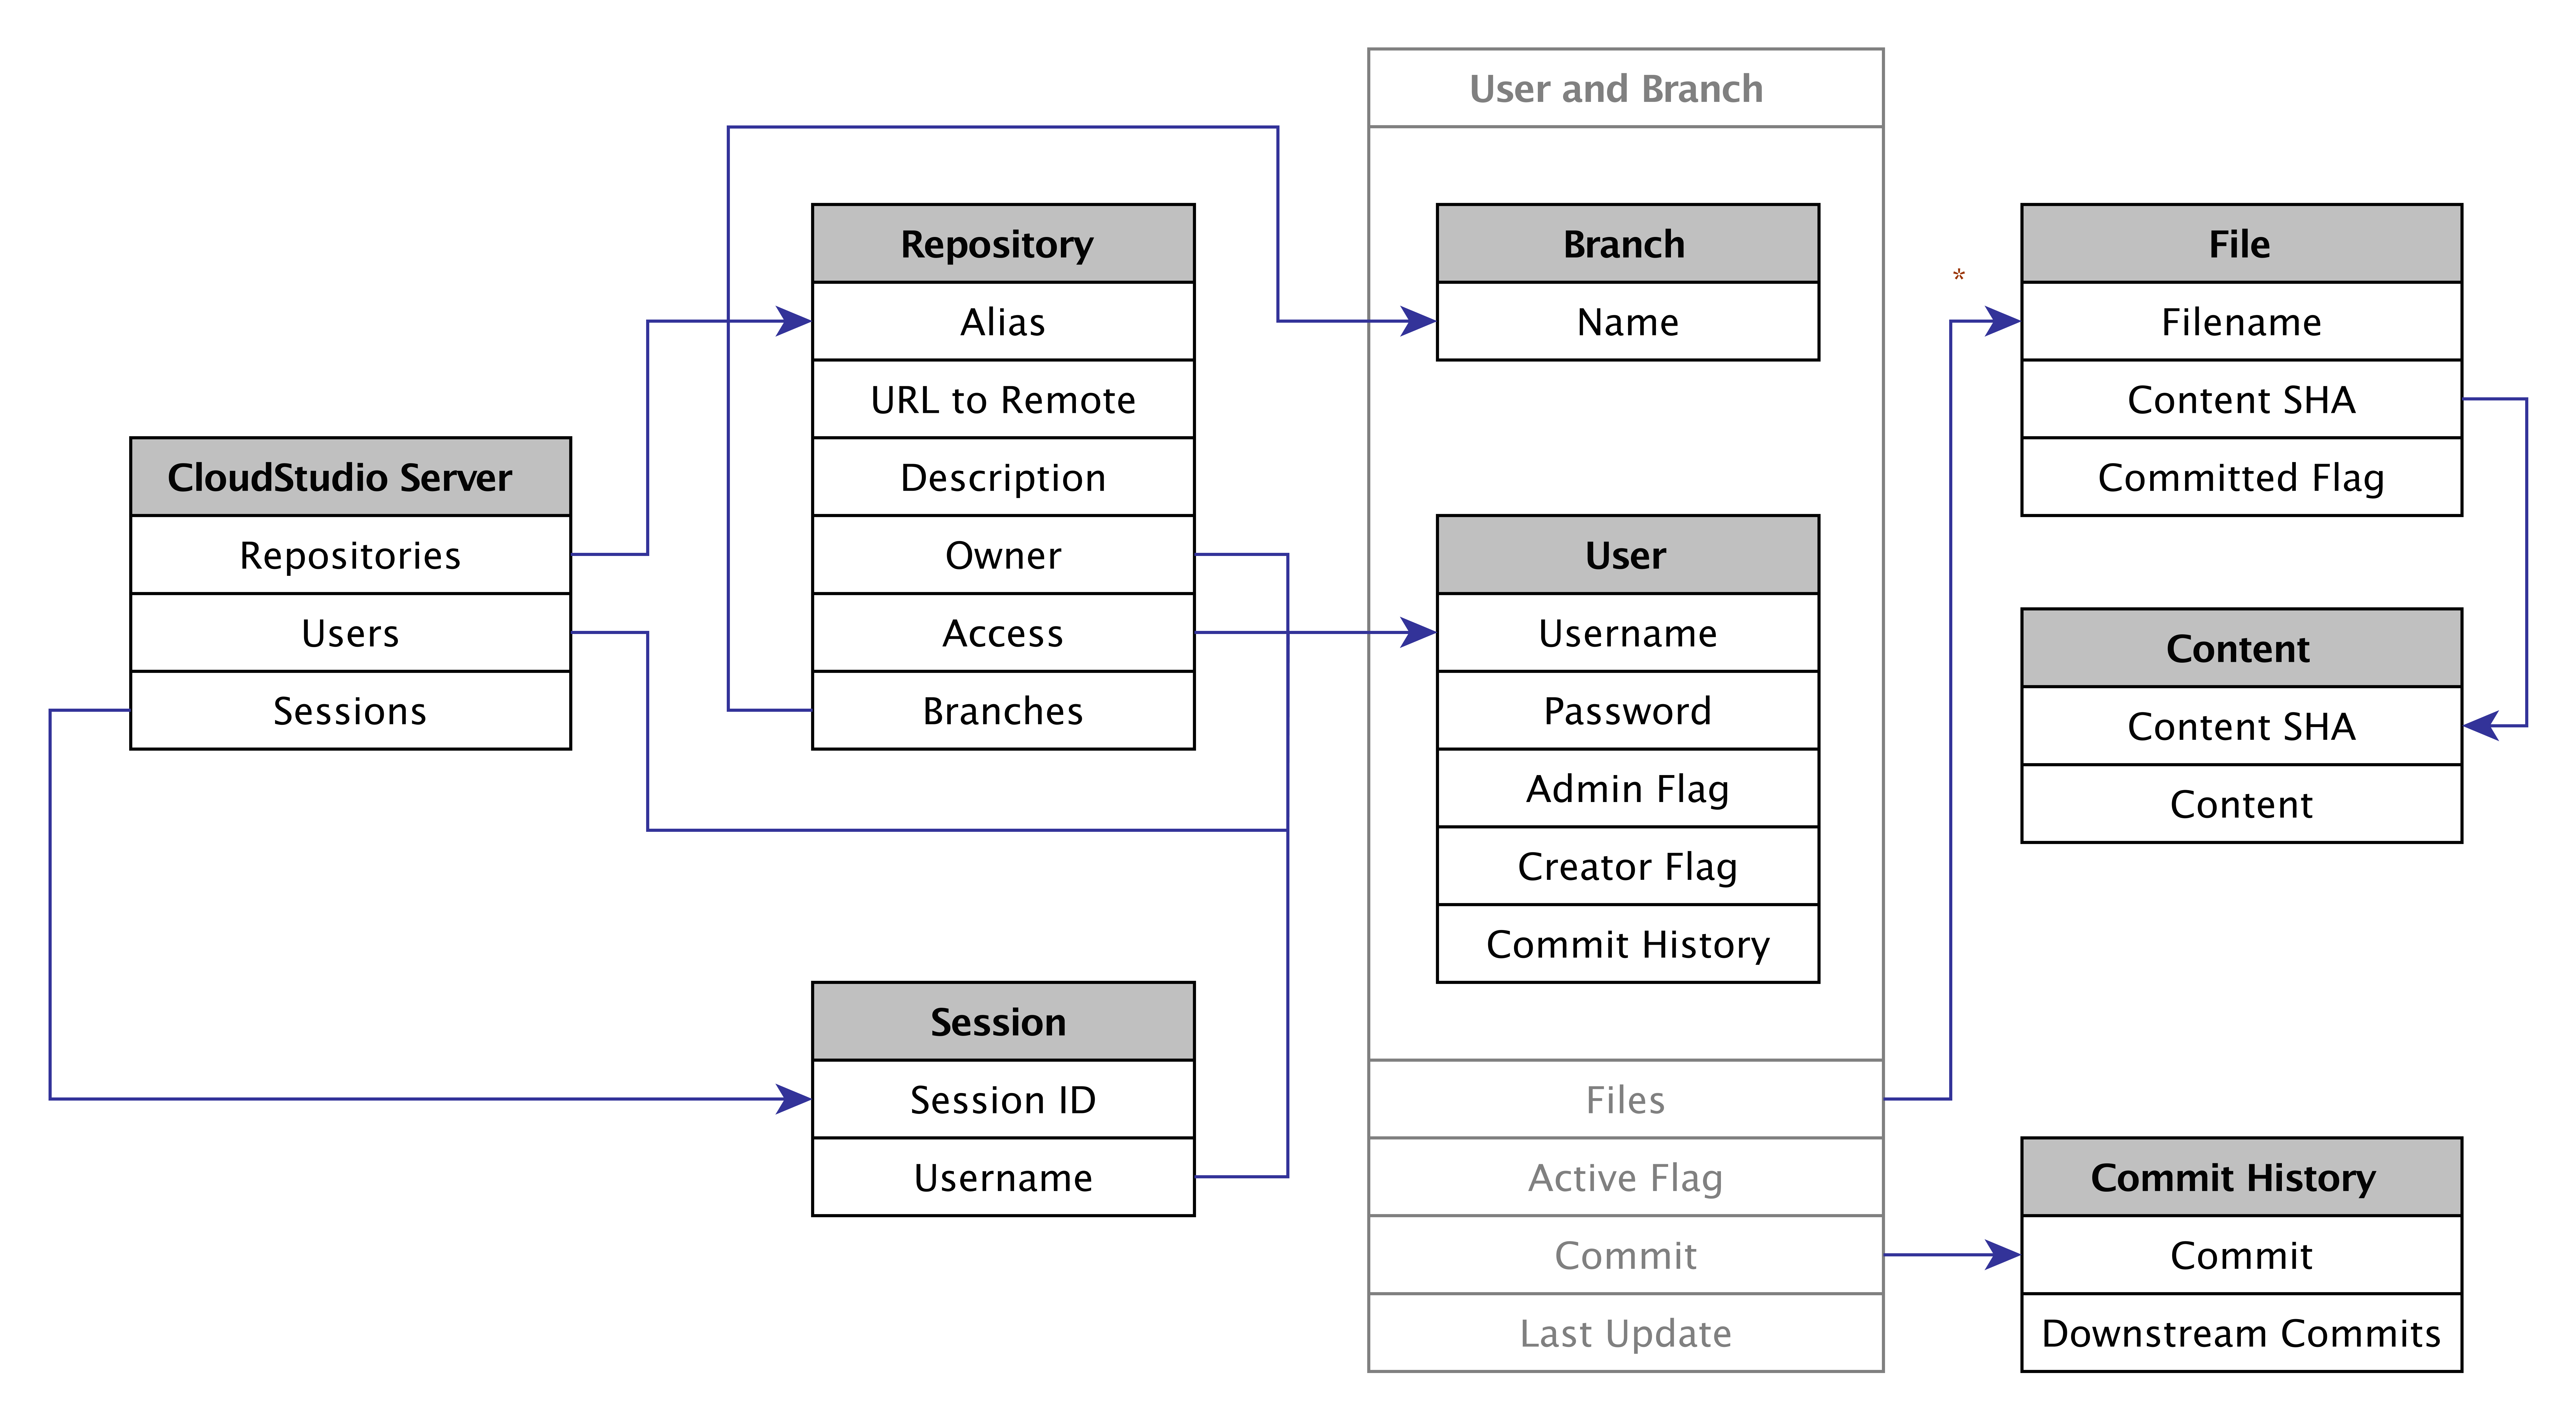
\includegraphics[width=1\textwidth]{entities}
  \caption{CloudStudio architecture}
  \label{fig:entities}
\end{figure}


The CloudStudio server primarily knows about users, repositories and sessions. \\

In order to do any sort of data manipulation or awareness requests, a user needs to request a session ID from the server via the $login$ API routine. This session ID will then be sent in every subsequent request to the server to verify a users authentication. A new user can also be created using the $createUser$ API command. \\

A user has a username, a password (that is hashed before storing it), an admin flag (determines whether a user has administrator privileges) and a creator flag (indicating the ability of a user to create new repositories). \\

Repositories refer to the internal CloudStudio entity of a shared Git repository. A repository has an alias (its internal and unique name in CloudStudio), a description, a URL to a remote repository (e.g. on GitHub), a list of users that have access to it and an owner (who can modify repository specific data, add or remove users, or delete the repository entirely). \\

For every user and branch in the repository, the information sent by the CloudStudio client is stored individually. On the level of a single repository, this means that every user has one or several branches that contain files, a (partial) commit graph, an active flag (indicating whether a user has currently checked out this branch into his working tree) and a timestamp when the user has last sent information about this branch to the CloudStudio server. \\

Files are represented as an object with a filename, a content SHA checksum and an committed value. The committed value can be one of three values: $committed$ (this exact file is currently part of a local commit), $uncommitted$ (this is the latest version of a file directly from the working directory) or $both$ (the uncommitted and committed files and contents are identical in this branch). \\

All of the above information is stored in the MySQL database, while the content of the files are stored in the filesystem, named by their SHA. The file object points to its content via the SHA. \\

A special user named "origin" is automatically added to the server and every repository and represents the central remote repository. It stores the Git information the same way a normal CloudStudio user would.

\subsection{Logic}

[TODO] \\

[TODO] \\

[TODO]

\subsection{Access Control}

CloudStudio provides a central login structure, which can be used by many users collaborating on different shared projects. Each repository has a designated owner who has the rights to add or remove people to the project, change its metadata, elect a new owner, or remove the repository all together. \\

Administrators can manage users and their privileges, as well as perform any actions that a repository owner or normal user could. A "creator" flag for each user indicates whether or not they have the privilege the create new repositories on CloudStudio. In the server configuration, you can enable or disable to set this flag by default for new users. In some closed environments, e.g. teachers set up projects for students and add them to the project, it may be preferred that not all users can create new repositories on CloudStudio.


\subsection{Folder Structure}

The source files are divided into 4 folders at the root level: $CSClient$ contains the client classes, $CSServer$ contains the server classes and the web interface, $CSCommon$ contains classes shared by client and server, and $CSTesting$ contains the JUnit tests used to verify CloudStudio's correctness.






\section{Client}

The client is responsible for periodically sending information for all the local Git repositories that are being monitored by CloudStudio. All users in a repository should use the CloudStudio client; however if only a subset of the users use it, awareness information is still prepared by the CloudStudio server. \\

The client is written in Java and uses JGit [18], a Java library to read and manipulate local Git repository information. It periodically retrieves local commit graph structure, branch references and files and their contents, for both uncommitted and committed files, and then sends relevant information to the CloudStudio server. This is done using a single API call $localState$ and the exact details can be found in the API Reference. Table \ref{table:clientclasses} shows the client's Java classes and quickly describes their function. The code for all individual classes is commented throughout. For detailed information, have a look at the source code. \\




\begin{table}

    \scriptsize
    \begin{tabularx}{\textwidth}{ | l | X | }
    \hline
\textbf{Class} & \textbf{Description} \\ \hline
ClientMain & This is the main class. It initiates reading the configuration file, launching the GUI, and periodically reading the local Git repositories and sending the gained information to the server. \\ \hline
ClientGUI & Renders the GUI elements using Swing. \\ \hline
HttpClient & Communicates with the CloudStudio server API using an HttpUrlConnection. \\ \hline
RepositoryReader & Reads a local repository using JGit and retrieves information relevant to CloudStudio's awareness capabilities. \\ \hline
ClientConfig & Container for configuration data. \\ \hline
RepositoryInfo & Container for repository data. \\ \hline
    \end{tabularx}
    
    \centering
  \caption{Client classes}
  \label{table:clientclasses}
\end{table}


Configuration of the client is done using an XML file. By default it looks for a file named \texttt{config.xml} in the same folder; alternatively, you can specify a config file location as the first command line parameter when running the client. In order to successfully use the client you need to first create a CloudStudio login and specify it in your configuration file. Configuration management of client and server is explained in detail in section \ref{configmanagement}. \\

To facilitate the users' experience, a graphical user interface (seen in Fig. \ref{fig:gui}), using Swing, keeps you informed using a virtual traffic light, indicating the state of the client, a progress bar to indicate the next time that information is pushed to the server, a force update button and a log view for more detailed information. A green light means everything functioning correctly, yellow indicates that some sort of error has occurred at some point but the system is still functioning (see the log view in the GUI for details), and a red light means that a hard error has occurred that the system could not recover from. At this point, the graphical user interface cannot be used to manipulate the configuration of the client. \\

\begin{figure}[h!]
  \centering
      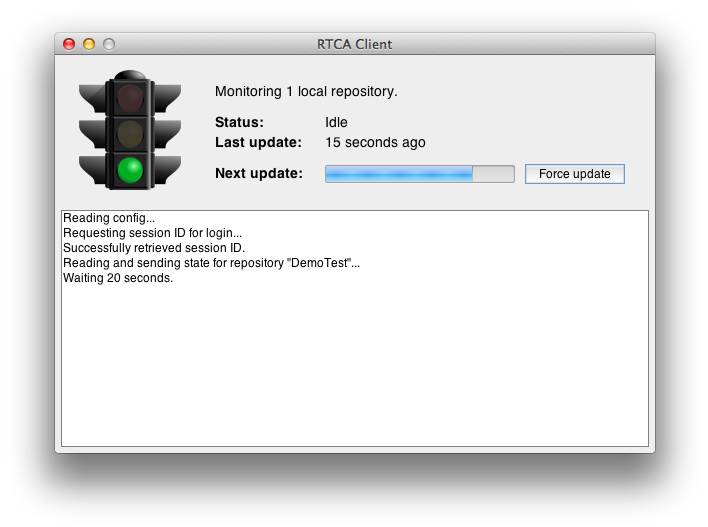
\includegraphics[width=0.8\textwidth]{gui}
  \caption{Screenshot of the CloudStudio client}
  \label{fig:gui}
\end{figure}








\section{Server}

The CloudStudio server is written in Java and is the core of the system. It reads, stores and processes information necessary for awareness requests and conflict detection. There are two main services running on the CloudStudio server: an HTTP server and a service to periodically update information from the central remote Git repositories used by CloudStudio projects. \\

The HTTP server implements the multi-threaded \texttt{com.sun.httpserver} and two separate request handlers deal with API requests and the web interface on the same port. The class ApiHttpHandler is responsible for calls to URLs prefixed with \texttt{/api/} and provides a public interface for the main CloudStudio server functionality. Any other URLs will be directed to the WebInterfaceHttpHandler, which is mostly just a static web server; the actual web interface runs in JavaScript and uses the API directly. Details about the implementations of the web interface follow in the next section. \\

PeriodicalAllOriginUpdater is the service to periodically update the remote repository information for all CloudStudio projects. Behind the curtains, it clones the given Git repositories and reads and stores them in the same manner as a regular client would. It uses the special user account "origin", which is added to all projects by default. Table \cite{fig:serverclasses} shows an overview of the server's Java classes. The code for all individual classes is commented throughout. For detailed information, have a look at the source code. \\

All CloudStudio data is stored in a MySQL database, accessed either directly through the JDBC driver or using the C3P0 database connection pool, depending on the server settings. \\

The server is greatly customizable through a configuration XML file, described in in section \ref{configmanagement}.


\begin{table}

    \scriptsize
    \begin{tabularx}{\textwidth}{ | l | X | }
    \hline
\textbf{Class} & \textbf{Description} \\ \hline
ApiHttpHandler & Handles HTTP exchanges for API requests. \\ \hline
ContentConflictGitReader & Finds the common ancestor needed to find conflicts and do three-way comparisons. \\ \hline
DatabaseConnection & Performs operations on the database. \\ \hline
DatabaseConnctionPool & Accesses and returns a data source from C3P0 database connection pool. \\ \hline
OriginUpdater & Updates remote Git repository information for a single repository and writes information into the database. \\ \hline
PeriodicalAllOriginUpdater & Periodically calls OriginUpdater with all the remote repositories used by CloudStudio projects. \\ \hline
ServerConfig & Reads the configuration file and returns individual parameters. \\ \hline
ServerMain & Main class that reads the config, sets up the origin updater and starts the HTTP server. \\ \hline
SideBySideDiff & Prepares a side-by-side comparison JSON object for two files. \\ \hline
SideBySideThreeWayDiff & Prepares a side-by-side compairson JSON object for a three-way comparison. \\ \hline
SqlQueryReader & Reads and caches SQL queries stored in external files. \\ \hline
WebInterfaceHttpHandler & Handles HTTP requests to the web interface. \\ \hline
ProcessWithTimeout & Helper class to allow a timeout for Process executions. \\ \hline
ParameterFilter & Helper class to parse HTTP GET and POST parameters. \\ \hline
    \end{tabularx}
    
    \centering
  \caption{Server classes}
  \label{table:serverclasses}
\end{table}



\section{Web Interface}

CloudStudio has a web interface that allows you to view awareness information from the browser. The web interface runs on the same server and port as the API. The logic of the web interface runs in JavaScript and on the client side; an approach that is popular with many web services nowadays. The server serves as a static webserver and awareness data is fetched directly through via the official CloudStudio API. \\

The CloudStudio web interface uses EJB, a light-weight templating engine, and jQuery, a fast, small, and feature-rich JavaScript library that makes thinks like HTML document manipulation, event handling, and Ajax much simpler. \\

The web interface was designed in a modern way, that it very user intuitive and easy to understand. The functionality of the web interface is explained in detail in section \ref{webinterfaceguide}.



\section{API}

The CloudStudio API exposes an interface to access and manipulate CloudStudio resources. All CloudStudio resources are accessed and manipulated in a similar way. Requests to the CloudStudio API have to use either the GET or POST method. GET requests are used for functions that do not change the state of the database. POST requests are used for functions that make changes to the database. \\

The content type of requests to the CloudStudio API must be \texttt{application/x-www-form-urlencoded}. The response has content type \texttt{application/json}. This asynchronism allows to provide parameters for both GET and POST requests similarly and still retrieve comprehensive JSON objects, and is used by many widely used APIs (e.g. SoundCloud). The entire API documentation can be found in the Appendix of this thesis or directly on the project's GitHub page.



\section{Database}\label{database}

The back-end for all data stored in the system is a MySQL database. The database is accessed using the JDBC driver directly, or using the C3P0 connection pool framework, depending on the configuration settings. Figure \ref{fig:databasegraph} shows the database tables and their primary (indicated as $PK$) and foreign keys (indicated as arrows). Table \ref{table:databasetables} explains the functionality of each table.


\begin{figure}[h!]
  \centering
      \includegraphics[width=0.8\textwidth]{databasegraph}
  \caption{CloudStudio's database setup}
  \label{fig:databasegraph}
\end{figure}



\begin{table}

    \scriptsize
    \begin{tabularx}{\textwidth}{ | l | X | }
    \hline
\textbf{Table} & \textbf{Description} \\ \hline
USERS & CloudStudio users \\ \hline
REPOSITORIES & every entry represents a CloudStudio repository \\ \hline
USERSESSION & every entry represents a session \\ \hline
USERACCESS & which user has access to a repository (n:n) \\ \hline
BRANCHES & branches for a user and repository \\ \hline
FILES & files for a user and repository, branch \\ \hline
COMMITHISTORY & commithistory for a user and repository \\ \hline
RepositoryInfo & container for repository data \\ \hline
    \end{tabularx}
    
    \centering
  \caption{Database tables}
  \label{table:databasetables}
\end{table}



\section{Configuration Management}\label{configmanagement}

\subsection{Client Configuration}

In order to run the client JAR, you need to have a configuration file called config.xml in the same directory. Alternatively, you can also specify the path to a config file as the first parameter. A sample configuration file looks like can be seen in Fig. \ref{fig:clientconfig}. \\

\begin{figure}[h!]
\begin{lstlisting}
 <?xml version="1.0" encoding="UTF-8"?>
 <config>
     <username>John</username>
     <password>burgers</password>
     <serverUrl>http://cloudstudio.ethz.ch:7330</serverUrl>
     <repositories>
         <repository>
             <alias>RepositoryAliasOnCloudStudio</alias>
             <localPath>/path/to/your/local/repository</localPath>
         </repository>
     </repositories>
     <resubmitInterval>300</resubmitInterval>
 </config>
\end{lstlisting}
  \centering
  \caption{Sample client configuration}
  \label{fig:clientconfig}
\end{figure}


Specify your $username$ and $password$ that you previously created for CloudStudio using its API or the web interface. Your user must have been added to the repository on CloudStudio. \\

Under repositories you can list multiple repositories that you want to monitor with CloudStudio. The $repositoryAlias$ is the name that a given repository has on CloudStudio and the $localPath$ is the folder where you locally cloned your Git repository into. Specify a time in seconds as the $resubmitInterval$, indicating how often the client sends data to the CloudStudio server.


\subsection{Server Configuration}

Figure \ref{fig:serverconfig} shows a sample configuration. Table \ref{table:serverconfigtable} explains what the individual parameters do. After setting up the configuration file, you need to run \texttt{SQLInit.sql} to initialize the database (MySQL), before starting the server.

\begin{figure}[h!]
\begin{lstlisting}
 <?xml version="1.0" encoding="UTF-8"?>
 <config>
     <serverPort>7330</serverPort>
     <dbDriverClass>com.mysql.jdbc.Driver</dbDriverClass>
     <dbJdbcUrl>jdbc:mysql://localhost/cloudstudio</dbJdbcUrl>
     <dbUser>dbadmin</dbUser>
     <dbPassword>1234</dbPassword>
     <useDatabasePool>true</useDatabasePool>
     <dbMinPoolSize>5</dbMinPoolSize>
     <dbAcquireIncrement>5</dbAcquireIncrement>
     <dbMaxPoolSize>20</dbMaxPoolSize>
     <dbMaxStatements>180</dbMaxStatements>
     <fileStorageDirectory>path/to/filestorage</fileStorageDirectory>
     <originStorageDirectory>path/to/origins</originStorageDirectory>
     <passwordSalt>GXSBML0EGjOMfqPzsznUCkK8ENP3lmOX</passwordSalt>
     <enableOriginUpdate>true</enableOriginUpdate>
     <originUpdateInterval>300</originUpdateInterval>
     <createAdminUser>true</createAdminUser>
     <giveCreatorPrivilegesOnSignUp>true</giveCreatorPrivilegesOnSignUp>
 </config>
\end{lstlisting}
  \centering
  \caption{Sample server configuration}
  \label{fig:serverconfig}
\end{figure}


\begin{table}

    \scriptsize
    \begin{tabularx}{\textwidth}{ | l | X | }
    \hline
\textbf{Setting} & \textbf{Description} \\ \hline
serverPort & Port for the HTTP server hosting the API and the Web Interface \\ \hline
dbDriverClass & JDBC driver \\ \hline
dbJdbcUrl & Database URL \\ \hline
dbUser & Database username \\ \hline
dbPassword & Database password \\ \hline
useDatabasePool & Enable C3P0 database pooling (\emph{true}/\emph{false}) \\ \hline
dbMinPoolSize & C3P0: minimum pool size \\ \hline
dbAcquireIncrement & C3P0: acquire increment \\ \hline
dbMaxPoolSize & C3P0: maximum pool size \\ \hline
dbMaxStatements & C3P0: maximum database statements \\ \hline
fileStorageDirectory & The database only stores file hashes. The file contents to the hashes are stored in this directory. \\ \hline
originStorageDirectory & A clone of the remote repository is stored in this directory for all projects. \\ \hline
passwordSalt & Salt for the password hash \\ \hline
enableOriginUpdate & Periodically fetch all remote repositories (\emph{true}/\emph{false}) \\ \hline
originUpdateInterval & How often to update remote repositories (in seconds) \\ \hline
createAdminUser & Create an administrator with username "Admin" and password "1234" if it doesn't exist on server start (\emph{true}/\emph{false})  \\ \hline
giveCreatorPrivilegesOnSignUp & Automatically give repository creation privileges when a new user is created (\emph{true}/\emph{false})  \\ \hline
    \end{tabularx}
    
    \centering
    
  \caption{Server configuration parameters}
  \label{table:serverconfigtable}
  
    \end{table}
    



\section{Testing and Correctness}

The Eclipse plugin EclEmma \cite{eclemma} was used to create coverage reports and view the line coverage directly in the workbench. EclEmma is a free code coverage tool, based on the JaCoCo \cite{jacoco} library. A high code coverage indicates that the code has been more thoroughly tested and there is a lower chance of software bugs than in a program with low code coverage \cite{codecoverage}. The coverage report created by EclEmma can be seen in Figure \ref{fig:testcoverage}. \\

To verify CloudStudio's correctness, I implemented two different types of JUnit \cite{junit} tests: $class$ $tests$ for client and server verify the correct behaviour for a given class and are named after the class that is being tested, e.g. ApiHttpHandlerTest for ApiHttpHandler; $combination$ $tests$ run longer scenarios of a typical CloudStudio workflow and assert correct behaviour throughout. \\

The CloudStudio client and server use the Apache Log4j \cite{log4j} framework to create log output; it can be customised by editing the log4j.xml file. Log files can as well be used to view and ensure the correct behaviour of the code.


\begin{figure}[h!]
  \centering
      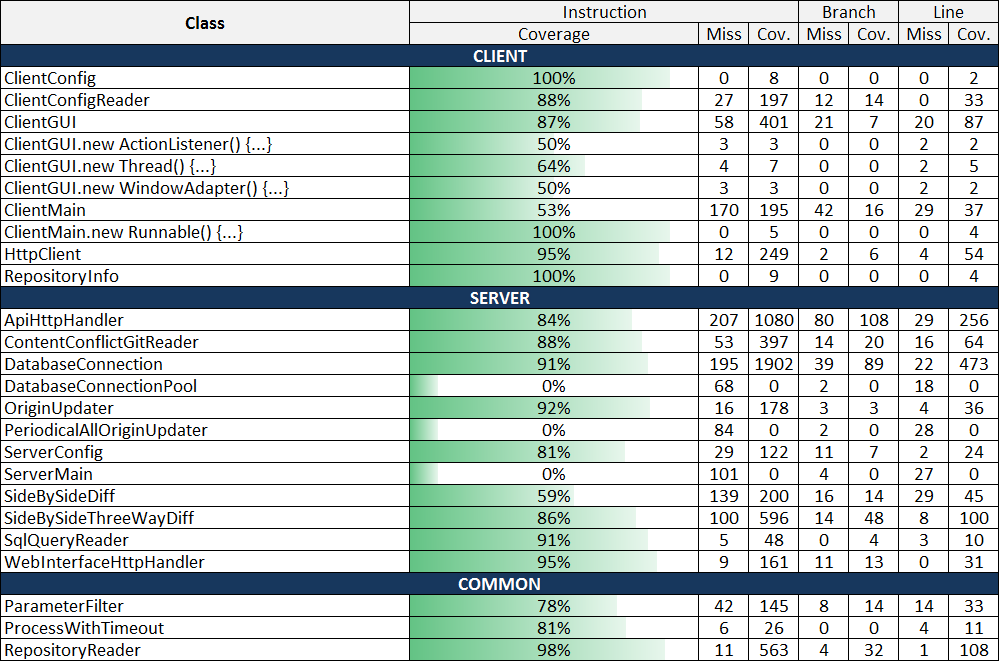
\includegraphics[width=0.9\textwidth]{coverage}
  \caption{Test coverage using EclEmma}
  \label{fig:testcoverage}
\end{figure}



\section{Build and Run}

Follow the following steps to build the CloudStudio server and client locally:

\begin{enumerate}


\item \emph{Clone the project.} \newline
\texttt{git clone https://github.com/fgremper/CloudStudio.git}
\item \emph{Import into Eclipse.} \newline Import the 4 folders CSClient, CSServer, CSCommon and CSTesting as existing Eclipse projects. (Open Eclipse and go to $File$ $\rightarrow$ $Import$ and select $Existing$ $Projects$ $into$ $Workspace$.)
\item \emph{Build JAR} \newline
In Eclipse, go to $File$ $\rightarrow$ $Export$ $\rightarrow$ $Java$ $\rightarrow$ $Runnable$ $JAR$ $file$.
Under $Launch$ $configuration$, select ClientMain to build the client JAR. To build the server JAR, select ServerMain. Under $Library$ $handling$, select $Package$ $required$ $libraries$ $into$ $generated$ $JAR$.
Select the export destionation and click Finish.
\item \emph{Run} \newline
Run the client:
\texttt{java -jar CSClient.jar} \newline
Run the server:
\texttt{java -jar CSServer.jar}

\end{enumerate}


%************************************************************************************
% Authors: Martin Nordio
% Date: March 2011
% Root file: report_root.tex
%************************************************************************************


%----------------------------------------------------------------------------
\chapter{User Guide}\label{userguide}
%----------------------------------------------------------------------------





\section{Setup and Run Client}

The fastest way to get started with CloudStudio is to use a precompiled client JAR directly from GitHub.

\begin{itemize}

\item Download the latest \texttt{CSClient.jar} directly from: \newline \texttt{http://github.com/fgremper/CloudStudio}

\item Go to \texttt{http://cloudstudio.ethz.ch:7330/} and create a new account by clicking "Sign up" in the top right corner and providing a new username and password.

\item Create a new config.xml file in the same directory as the client JAR you downloaded and paste in the setup configuration.

\item Replace the username and password with your username and password you just created.

\item If you want to work with an existing CloudStudio project, provide its repository alias and the path to your local Git repository, and make sure the repository owner adds you to the repository access list.

\item If you want set up a new CloudStudio project, click "Create repository" in the repository overview and provide an alias, description and possible an URL to a remote repository. Use the repository alias in your configuration file.

\item You can use the client to monitor multiple repositories with the same CloudStudio user account.

\end{itemize}

\section{Using the Web Interface}\label{webinterfaceguide}


%************************************************************************************
% Authors: Martin Nordio
% Date: March 2011
% Root file: report_root.tex
%************************************************************************************


%----------------------------------------------------------------------------
\chapter{Future Work}\label{futurework}
%----------------------------------------------------------------------------

The functionality integrated by this thesis can be easily extended. \\

While CloudStudio performed sufficiently in test projects, there are many steps that can be taken to improve its overall performance. To load the file level awareness view with conflict detection, a lot of file comparisons have to be made and files (common ancestors) have to be looked up through JGit. The results of operations like these could be cached to speed up the service. \\

CloudStudio offers an API that opens up the possibility to write all sorts of plugins that benefit from its awareness and conflict detection capabilities. Aside from using it directly through the web interface, future work can include writing plugins that directly display awareness information in a programmers preferred IDE. \\

As of this time, the client sends its entire information to the server every periodical update. It was a conscious decision not to send incremental one-way updates from the client to preserve stability of the system. However, it is conceivable to implement a delta update function where client and server negotiate what information has to be sent in order to lower the bandwidth requirements. \\

Git treats every commit as a snapshot, and as such is unaware of file renaming. It does however use heuristics to calculate the likelihood of a file rename given the similarity of two files. CloudStudio has not yet implemented any heuristics to detect file renames and would greatly benefit from doing so. \\

The Chair of Software Engineering at ETH Zurich has been teaching a "Distributed and Outsourced Software Engineering" (DOSE) course for several years to prepare student for new challenges in a distributed development environment. \cite{ref19, ref20} CloudStudio can be used as a means of collaboration and to heighten the sense of awareness in student projects, by both students and the teaching assistants.





%************************************************************************************
% Authors: Martin Nordio
% Date: March 2011
% Root file: report_root.tex
%************************************************************************************


%----------------------------------------------------------------------------
\chapter{Conclusions}\label{conclusions}
%----------------------------------------------------------------------------






Software engineering is becoming increasingly distributed activity. Teams are spread out over all of the world and new problems such as the lack of communication and awareness information arise, which may disrupt progress and jeopardise efficiency and timeliness \cite{ref3}. \\

CloudStudio proposes a new mechanism for making awareness information available and detect conflicts early on. One of the key features of CloudStudio is the opening of its functionality to developers by providing a public and well-documented API. This allows for integration of CloudStudio's awareness information into new services and common IDEs. CloudStudio acts as a separate layer on top existing Git projects and as such can be added at any time and no specific structure of the Git repository is required. \\

For the implementation of CloudStudio numerous feature requirements have been set from the start, listed under \ref{designfeatures}. This has been done in order to make sure that the information generated by CloudStudio is useful and accurate. The criteria for success have been specified in a project plan before starting the thesis and have been tightly followed. Furthermore, many new features and a beautiful web interface have been added. \\

Among the big challenges of the thesis were the distributed nature of the project and making sure all the individual parts work together smoothly, studying the structure of Git and coming up with an awareness system that is useful, realisable and uses the available information from Git repositories. Also, the focus on stability and good error handling required a lot of testing and fixing small bugs. \\

Many extensions to the existing version of CloudStudio are conceivable, some of which are listed in Chapter 5. CloudStudio offers an ideal platform for the "Distributed and Outsourced Software Engineering" (DOSE) course, allowing students to experiment with new sources of awareness information and hopefully improving the workflow of all participants.






%\bibliographystyle{abbrv}

%\bibliography{literatur}

% 11->2
% 7->6
% 16-10

\begin{thebibliography}{99}

\bibitem{ref1}
  Martin Nordio, Roman Mitin and Bertrand Meyer. \textbf{Advanced Hands-on Training for Distributed and Outsourced Software Engineering}, In Proceedings of the 32nd ACM/IEEE International Conference on Software Engineering - Volume 1, ACM. 2010.

\bibitem{ref2}
  E. Carmel. \textbf{Global software teams: collaborating across borders and time zones}. Prentice Hall PTR, Upper Saddle River, NJ, USA, 1999.

\bibitem{ref3}
  \textbf{Awareness and Merge Conflicts in Distributed Software Development}. H.-Christian Estler, Martin Nordio, Carlo A. Furia, Bertrand Meyer, In Proceedings of the 9th International Conference on Global Software Engineering (ICGSE) (Yuanfang Cai, Jude Fernandez, Wenyun Zhao, eds.), IEEE Computer Society, 2014.

\bibitem{ref4}
  Y. Brun, R. Holmes, M. Ernst, and D. Notkin. \textbf{Proactive detection of collaboration conflicts}. In ESEC/FSE, pages 168-178. ACM, 2011.

\bibitem{ref5}
  C. Bird, N. Nagappan, P. Devanbu, H. Gall, and B. Murphy. \textbf{Does distributed development affect software quality? An empirical case study of Windows Vista}. In Proceedings of the 31st International Conference on Software Engineering, ICSE ?09, pages 518-528, Washington, DC, USA, 2009. IEEE Computer Society.

\bibitem{ref6}
  J. Herbsleb and a. Mockus. \textbf{An empirical study of speed and communication in globally distributed software development}. IEEE Transactions on Software Engineering, 29(6):481-494, June 2003.

\bibitem{ref8}
  J. A. Espinosa, N. Nan, and E. Carmel. \textbf{Do Gradations of Time Zone Separation Make a Difference in Performance? A First Laboratory Study}. In International Conference on Global Software Engineering (ICGSE 2007), pages 12-22. IEEE, Aug. 2007.

\bibitem{ref9}
  Martin Nordio, Roman Mitin, Bertrand Meyer, Carlo Ghezzi, Elisabetta Di Nitto and Giordano Tamburelli. \textbf{The Role of Contracts in Distributed Development}. In proceedings of Software Engineering Advances For Offshore and Outsourced Development (SEAFOOD), Lecture Notes in Business Information Processing 35, Springer-Verlag, 2009.

\bibitem{ref10}
  M. Nordio, H.-C. Estler, B. Meyer, J. Tschannen, C. Ghezzi, and E. D. Nitto. \textbf{How do distribution and time zones affect software development? A case study on communication.} In Proceedings of the IEEE International Conference on Global Software Engineering (ICGSE 2011). IEEE, 2011.

\bibitem{ref12}
  \textbf{Unifying Configuration Management with Awareness Systems and Merge Conflict Detection}. H.-Christian Estler, Martin Nordio, Carlo A. Furia, Bertrand Meyer, In 22nd Australasian Software Engineering Conference (ASWEC), IEEE, 2013.

\bibitem{ref13}
  \textbf{Collaborative Debugging}. H.-Christian Estler, Martin Nordio, Carlo A. Furia, Bertrand Meyer, In 8th International Conference on Global Software Engineering (ICGSE), IEEE, 2013.

\bibitem{ref14}
  J. A. Espinosa, N. Nan, and E. Carmel. \textbf{Do gradations of time zone separation make a difference in performance? A first laboratory study}. In Proceedings of the IEEE International Conference on Global Software Engineering (ICGSE 2007), pages 12-22. IEEE, Aug. 2007.

\bibitem{ref15}
  H.-C. Estler, M. Nordio, C. A. Furia, B. Meyer, and J. Schneider. \textbf{Agile vs. structured distributed software development: A case study}. In Proceedings of the 7th International Conference on Global Software Engineering. IEEE, 2012.

\bibitem{ref17}
  \textbf{Analysis of Git and Mercurial}. \newline https://code.google.com/p/support/wiki/DVCSAnalysis

\bibitem{ref18}
  \textbf{JGit}. http://eclipse.org/jgit/

\bibitem{ref19}
  Martin Nordio, Carlo Ghezzi, Bertrand Meyer, Elisabetta Di Nitto, Giordano Tamburrelli, Julian Tschannen, Nazareno Aguirre, Vidya Kulkarni. \textbf{Teaching Software Engineering using Globally Distributed Projects: the DOSE course}, In Collaborative Teaching of Globally Distributed Software Development - Community Building Workshop (CTGDSD), ACM, 2011.

\bibitem{ref20}
  Martin Nordio, Roman Mitin and Bertrand Meyer. \textbf{Advanced Hands-on Training for Distributed and Outsourced Software Engineering}, In Proceedings of the 32nd ACM/IEEE International Conference on Software Engineering - Volume 1, ACM. 2010.

\bibitem{ref21}
  K. Dullemond and B. van Gameren. \textbf{What distributed software teams need to know and when: An empirical study}. In ICGSE, pages 61-70, 2013.

\bibitem{ref22}
  A. Sarma, G. Bortis, and A. van der Hoek. \textbf{Towards supporting awareness of indirect conflicts across software configuration management workspaces}. In ASE, pages 94-103. ACM, 2007.

\bibitem{ref23}
  L. Hattori and M. Lanza. Syde. \textbf{A tool for collaborative software development}. In Proceedings of the 32nd ACM/IEEE International Conference on Software Engineering, pages 235-238. ACM Press, 2010.

\bibitem{ref24}
  L. Hattori, M. Lanza, and M. D'Ambros. \textbf{A qualitative analysis of preemptive conflict detection}. Technical Report 2011/05, University of Lugano, Sept. 2011.

\bibitem{ref25}
  Y. Brun, R. Holmes, M. Ernst, and D. Notkin. \textbf{Proactive detection of collaboration conflicts}. ESEC FSE, Szeged, Hungary, 2011.

\bibitem{ref26}
  J. Biehl, M. Czerwinski, G. Smith, and G. Robertson. \textbf{Fastdash: a visual dashboard for fostering awareness in software teams}. In Proceedings of the SIGCHI conference on Human factors in computing systems, CHI ?07, pages 1313-1322, New York, NY, USA, 2007. ACM.

\bibitem{ref27}
  S. Hupfer, L.-T. Cheng, S. Ross, and J. Patterson. \textbf{Introducing collaboration into an application development environment}. In Proceedings of the 2004 ACM conference on Computer supported cooperative work, CSCW ?04, pages 21-24. ACM, 2004.

\bibitem{ref28}
  \textbf{Automatic Version Control System for Distributed Software Development}. Sandra Weber, ETH Zurich, 2012
  
\bibitem{eclemma}
  \textbf{EclEmma}, http://www.eclemma.org/
  
\bibitem{jacoco}
  \textbf{JaCoCo}, http://www.eclemma.org/jacoco/
  
\bibitem{codecoverage}
  \textbf{Code Coverage}, http://en.wikipedia.org/wiki/Code\_coverage
    
\bibitem{log4j}
  \textbf{Apache Log4j}, http://logging.apache.org/log4j/2.x/
  
\bibitem{junit}
  \textbf{JUnit}, http://junit.org/
    
\end{thebibliography}


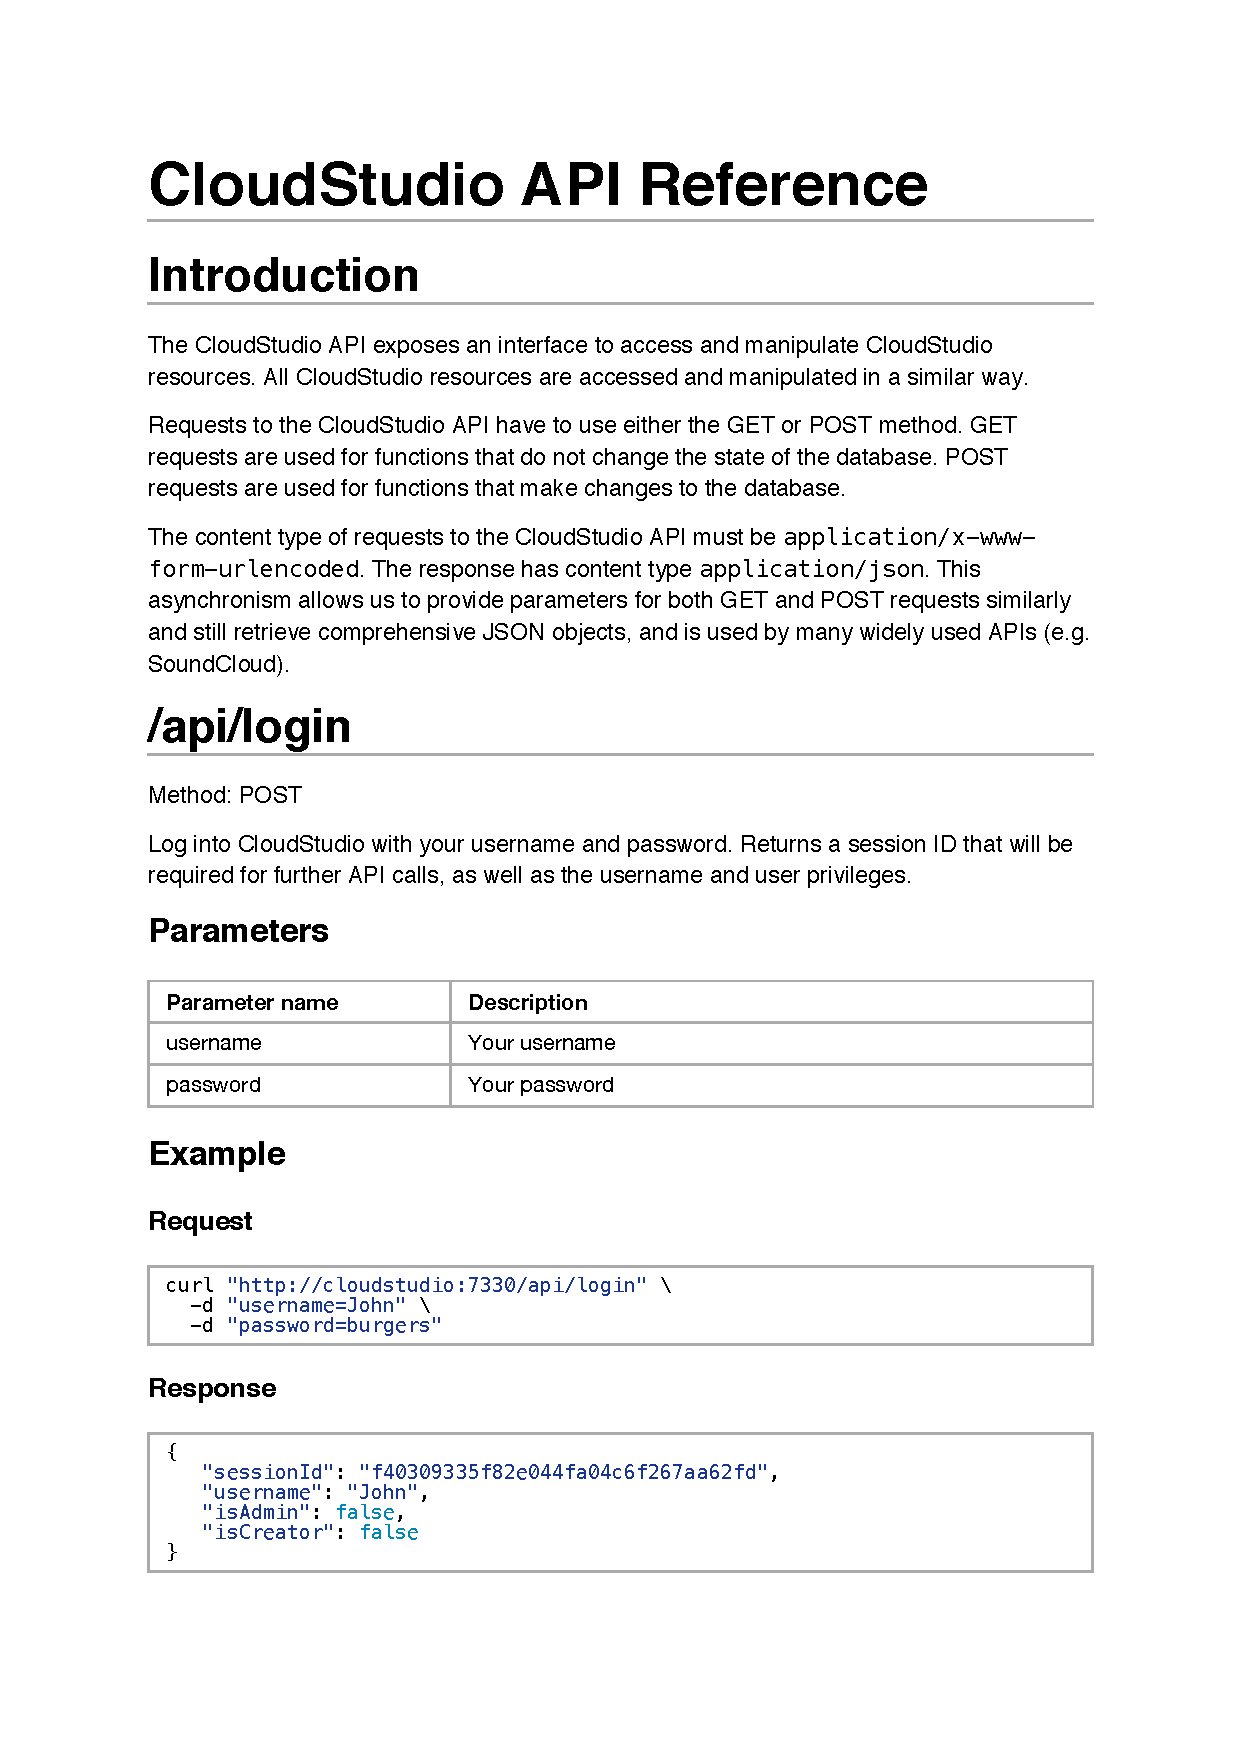
\includepdf[pages=-]{api.pdf}

\end{document}



